%\documentclass[table]{article}
%\usepackage{beamerarticle}
\documentclass[10pt,xcolor=table,ignorenonframetext,handout,aspectratio=169]{beamer}
%\documentclass[10pt,xcolor=table,ignorenonframetext]{beamer}
\mode<presentation>
{
  \usetheme{default}
  \useoutertheme{split}
% \usefonttheme{serif}
}

\usenavigationsymbolstemplate{}
\usepackage{amssymb}
\usepackage{amsmath}
\usepackage{setspace}
\usepackage{graphicx}
\usepackage{multirow}
\usepackage[english]{babel}
\usepackage[latin1]{inputenc}
\usepackage{bm}
\usepackage{graphicx}
\usepackage{multirow}
\usepackage{tikz}
\usepackage[english]{babel}
\usepackage[latin1]{inputenc}
%\usepackage{ulem}
\usepackage{pifont}
\usepackage{changepage}
%\usepackage{colortbl}
%\usepackage[table]{xcolor}
%\usepackage{xcolor}

\setbeamersize{text margin left=1cm,text margin right=1.2cm}

\setbeamertemplate{itemize item}[circle]
\setbeamertemplate{frametitle}[default][center]

\newlength{\wideitemsep}
\setlength{\wideitemsep}{\itemsep}
\addtolength{\wideitemsep}{4pt}
\let\olditem\item
\renewcommand{\item}{\setlength{\itemsep}{\wideitemsep}\olditem}

\newcommand{\HRule}{\rule{0.5\textwidth}{0.05mm}}

\usetikzlibrary{arrows,positioning,shapes}
\usetikzlibrary{decorations.pathreplacing}

\definecolor{blueish}{RGB}{97,156,255}
\definecolor{greenish}{RGB}{0,186,56}
\definecolor{reddish}{RGB}{248,118,109}

\definecolor{oiverm}{RGB}{213,94,0}
\definecolor{oiblue}{RGB}{0,114,178}
\definecolor{oigreen}{RGB}{0,158,115}
\definecolor{oipurple}{RGB}{204,121,167}
\definecolor{oiorange}{RGB}{230,159,0}
\definecolor{oisky}{RGB}{86,180,233}
\definecolor{oiyellow}{RGB}{240,228,66}
\definecolor{williams}{RGB}{81,38,152}

\definecolor{hue1}{RGB}{255,255,204}
\definecolor{hue2}{RGB}{161,218,180}
\definecolor{hue3}{RGB}{65,182,196}
\definecolor{hue4}{RGB}{44,127,184}
\definecolor{hue5}{RGB}{37,52,148}

\definecolor{dvg1}{RGB}{213,62,79}
\definecolor{dvg2}{RGB}{244,109,67}
\definecolor{dvg3}{RGB}{253,174,97}
\definecolor{dvg4}{RGB}{254,224,139}
\definecolor{dvg5}{RGB}{230,245,152}
\definecolor{dvg6}{RGB}{171,221,164}
\definecolor{dvg7}{RGB}{102,194,165}
\definecolor{dvg8}{RGB}{50,136,189}

\setbeamercolor{structure}{fg=williams,bg=williams!12}

\title{Why Evaluate? Slide \insertframenumber}
\subtitle{}

\author{Economics 379 (Professor Jakiela)}
\date{}



\begin{document}
	
	
	
%%%%%%%%%%%%%%%%%%%%%%%%%%%%%%%%%%%%%%%%%%%%%%%%%%%%%%%%%%%%%%%%%%%%%%%%%%
	% COURSE Title slide
%%%%%%%%%%%%%%%%%%%%%%%%%%%%%%%%%%%%%%%%%%%%%%%%%%%%%%%%%%%%%%%%%%%%%%%%%%
	
\begin{frame}<beamer:0>[plain]
	
	\begin{center}
		\begin{tikzpicture}
		
		\node [opacity=1] (bg)  {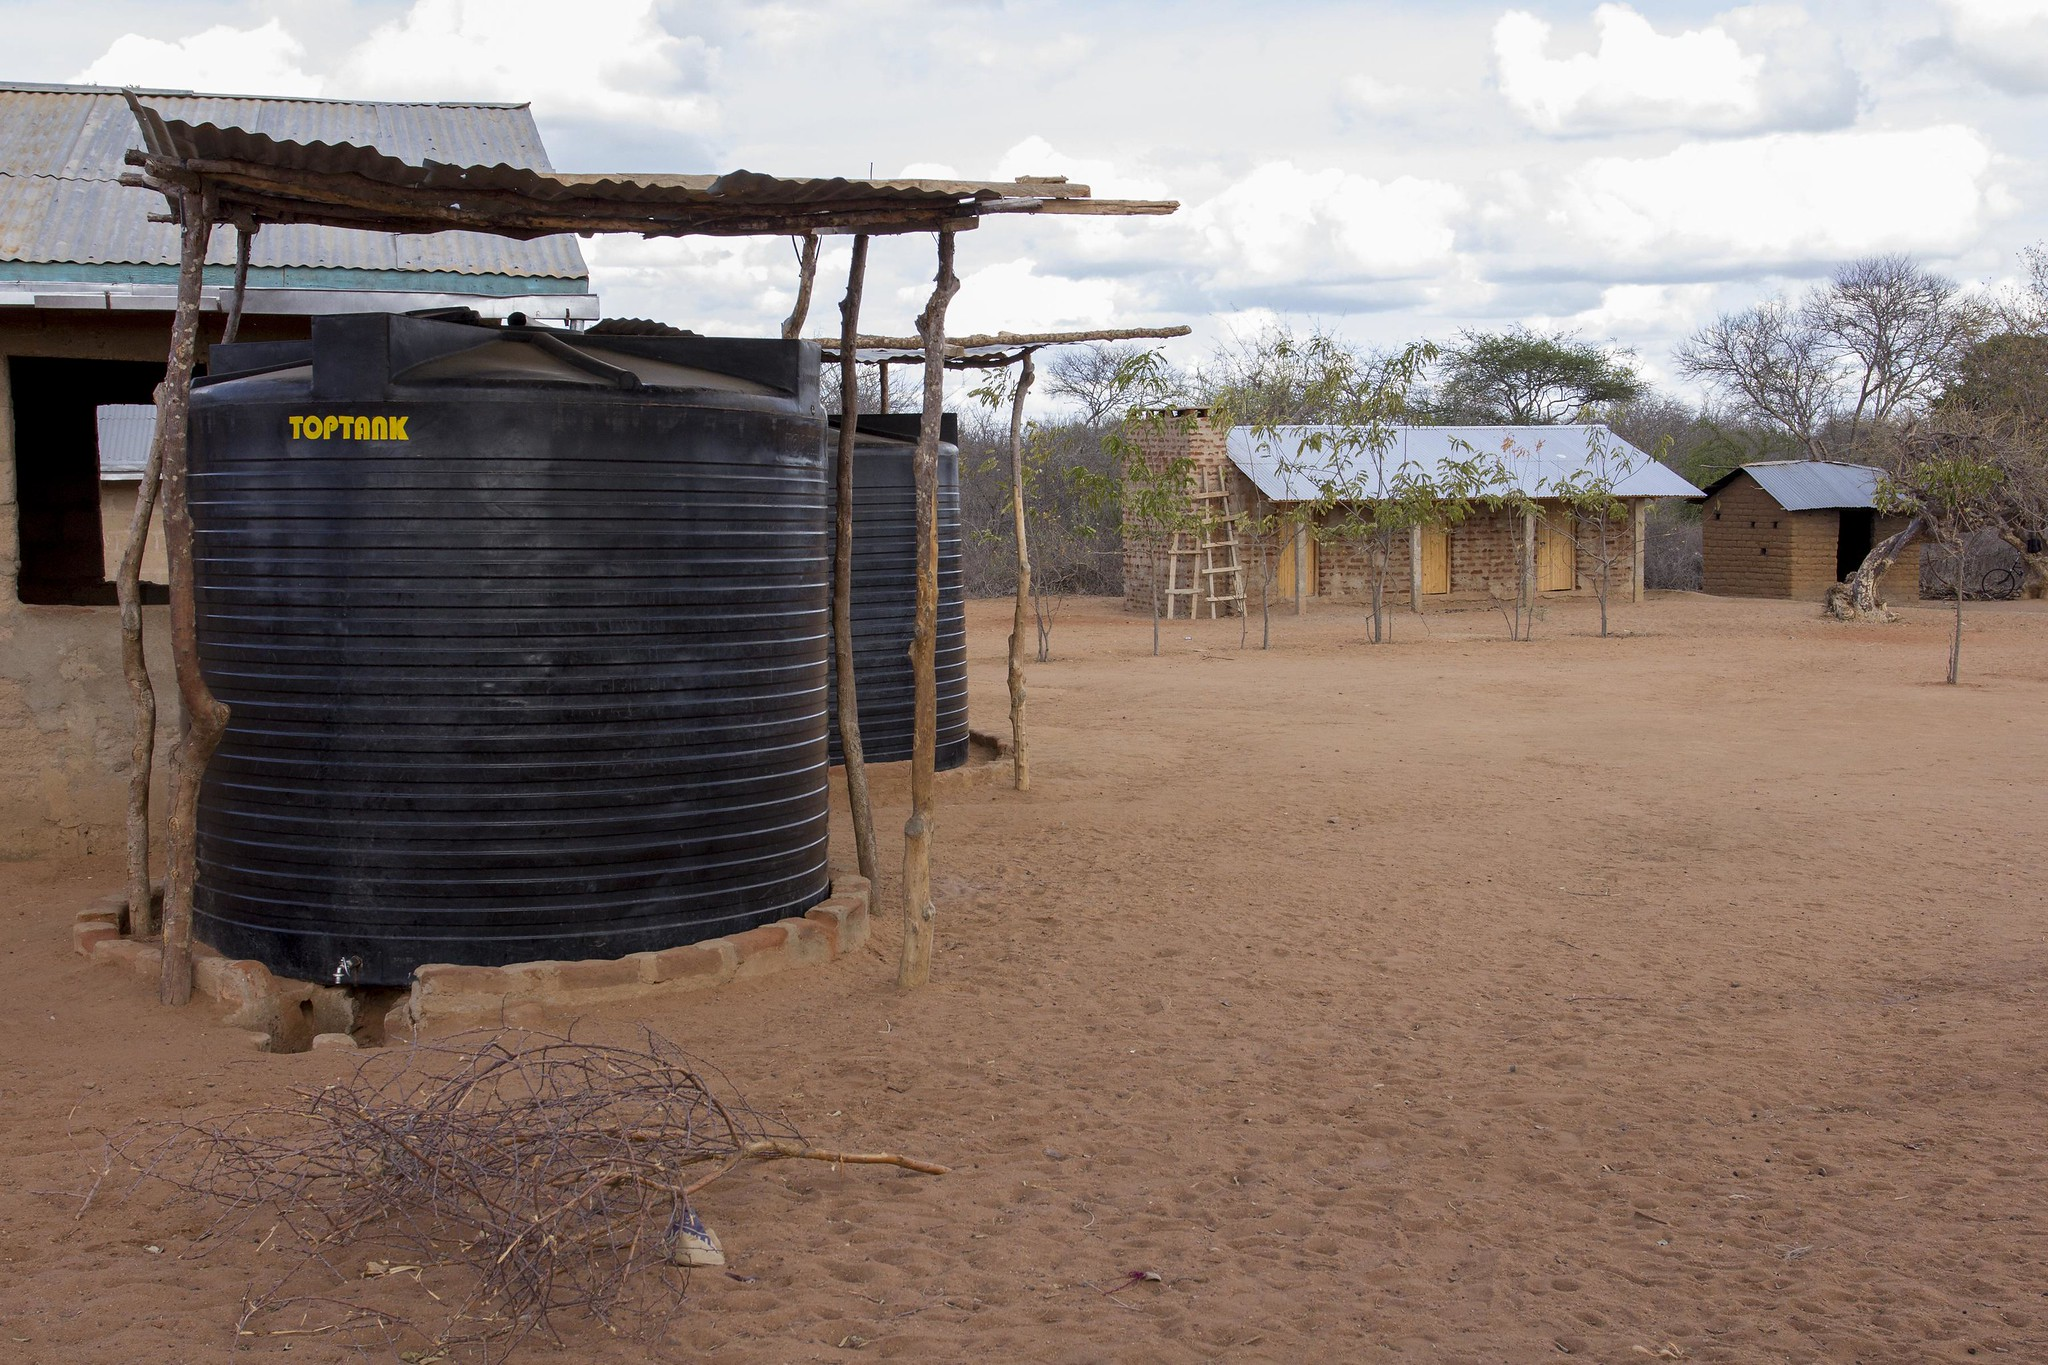
\includegraphics[keepaspectratio,height=0.9\paperheight]{photos/Kenya-cistern-Flore-de-Preneuf-2011-LARGE.jpg}};
		
		\node [anchor=east,align=right] at (6,-2.25) {\Large{\textcolor{white}{Williams College ECON 379:}}};		
		\node [anchor=east,align=right] at (6,-3) {\Large{\textcolor{white}{Program Evaluation for International Development}}};

		\node [anchor=east] at (6,-3.8) {\textcolor{yellow}{\tiny{photo:  Flore de Preneuf / World Bank}}};
		
		\end{tikzpicture}
	\end{center}
\end{frame}


%%%%%%%%%%%%%%%%%%%%%%%%%%%%%%%%%%%%%%%%%%%%%%%%%%%%%%%%%%%%%%%%%%%%%%%%%%
% LECTURE Title slide
%%%%%%%%%%%%%%%%%%%%%%%%%%%%%%%%%%%%%%%%%%%%%%%%%%%%%%%%%%%%%%%%%%%%%%%%%%

\begin{frame}[plain]

%\only<beamer>{\begin{adjustwidth}{0cm}{-4cm}}

\begin{center}
	\begin{tikzpicture}
	
	\node [opacity=0.25] (bg)  {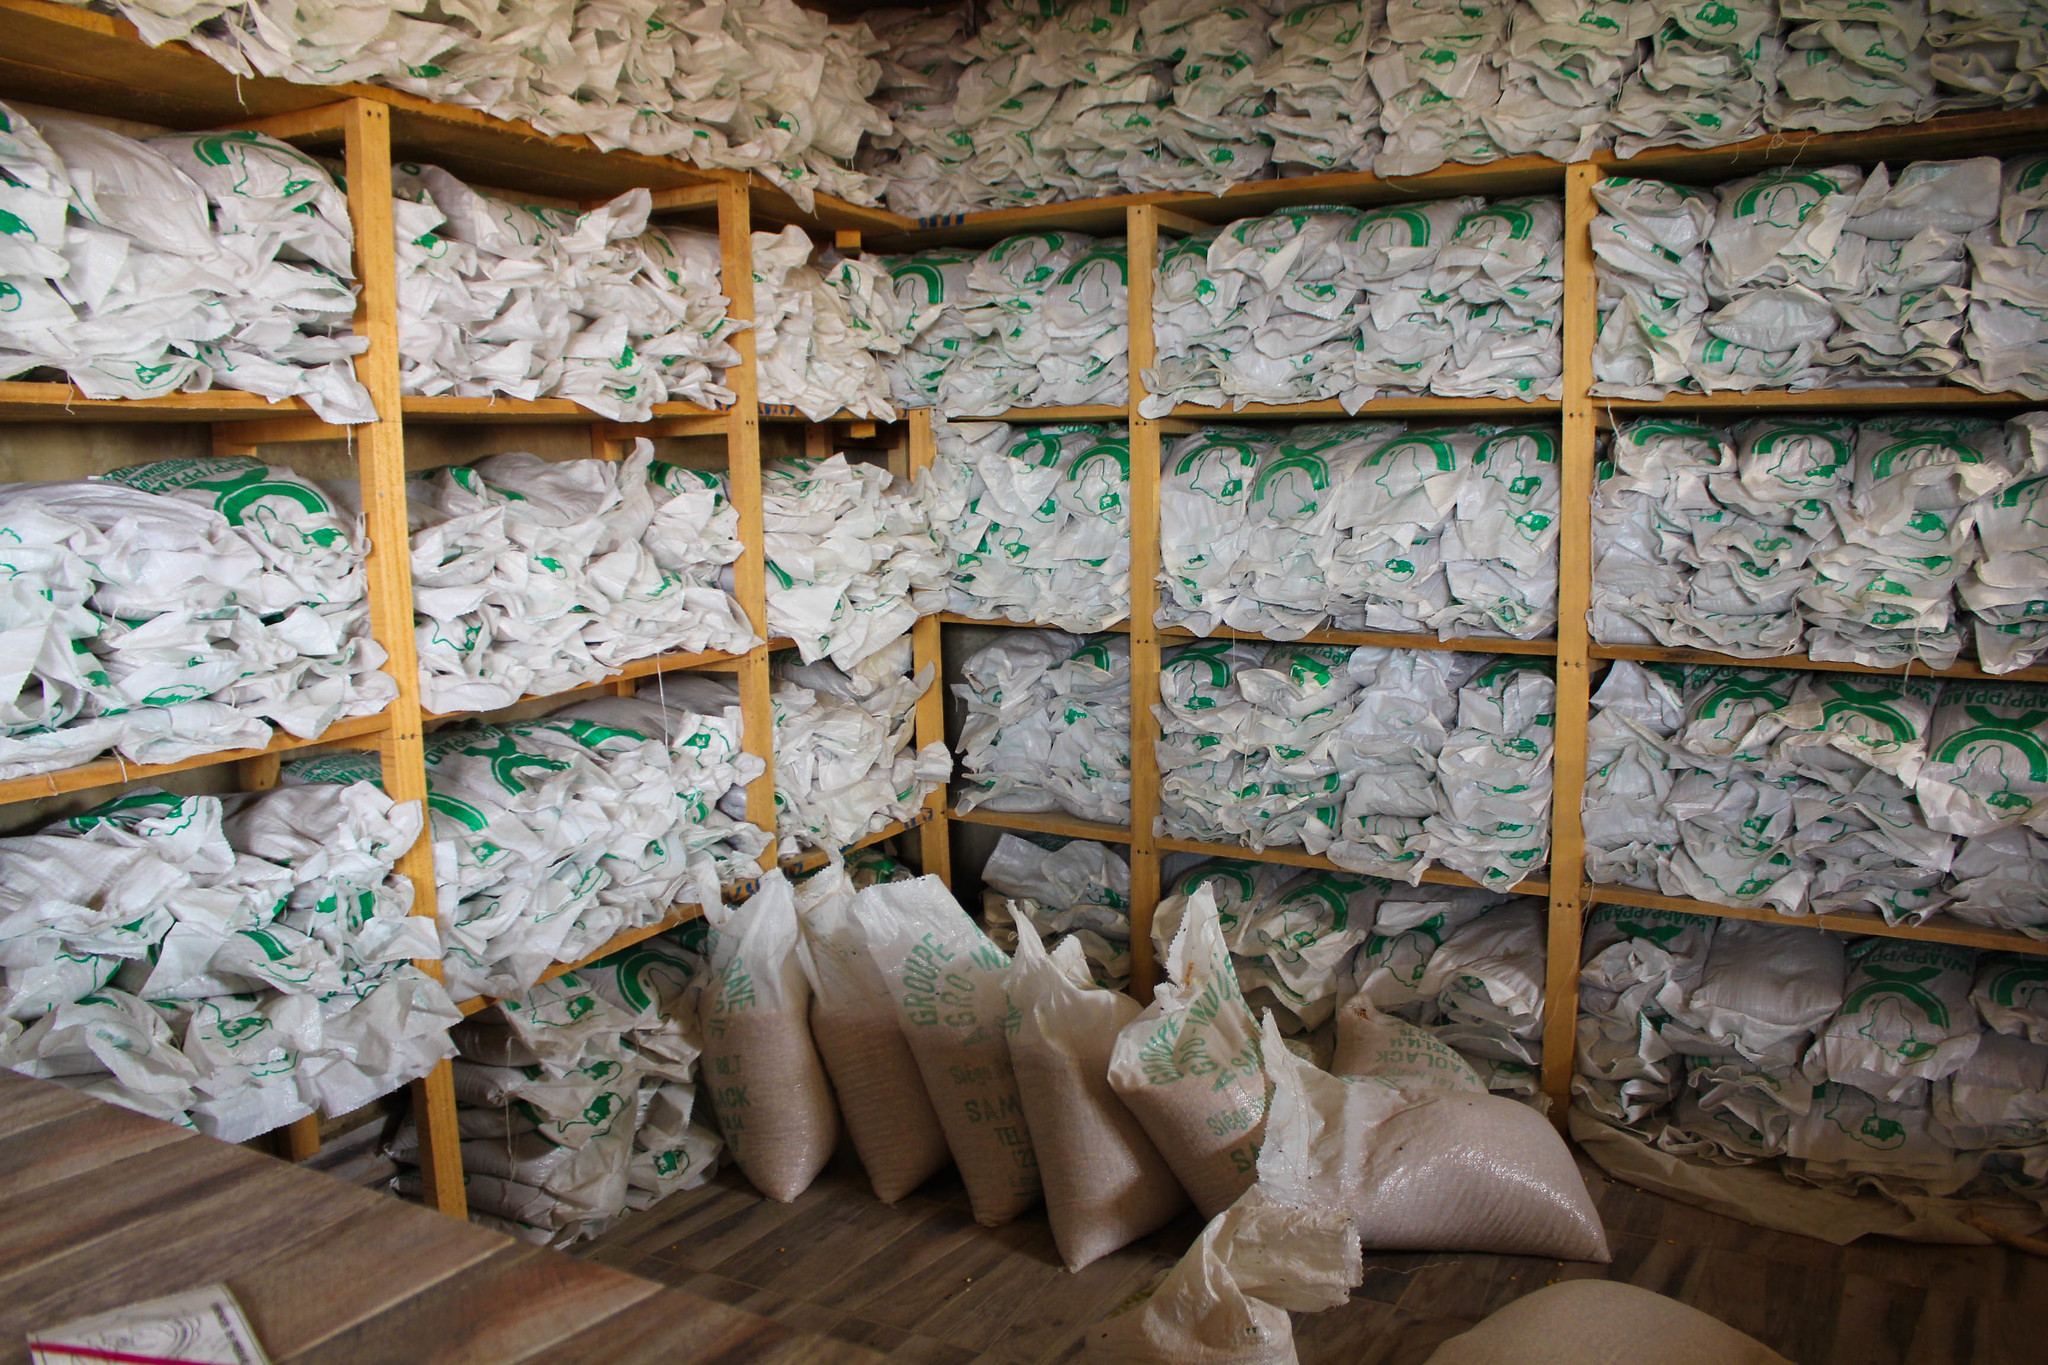
\includegraphics[keepaspectratio,height=0.9\paperheight]{photos/Senegal-WAAPP-seeds-Daniella-Van-Leggelo-Padilla-LARGE.jpg}};
	
	\node at (0,2.5) {\large{\textcolor{williams}{Williams College ECON 379:}}};		
	\node at (0,1.5) {\large{\textcolor{williams}{Program Evaluation for International Development}}};
	
	\node at (0,-0.5) {\large{\textcolor{williams}{\textbf{Module 1: Why Should We Evaluate Development Policy?}}}};
	
	\node at (0,-2) {\large{\textcolor{williams}{Professor:  Pamela Jakiela}}};
	
	\node [anchor=east] at (6,-3.8) {\textcolor{yellow}{\tiny{photo:  Daniella Van Leggelo-Padilla / World Bank}}};
	
	\end{tikzpicture}
\end{center}
%\only<beamer>{\end{adjustwidth}}
\end{frame}



%%%%%%%%%%%%%%%%%%%%%%%%%%%%%%%%%%%%%%%%%%%%%%%%%%%%%%%%%%%%%%%%%%%%%%%%%%%

%\begin{frame}<handout:0>[bg,plain]
\begin{frame}[plain]

%\only<beamer>{\begin{adjustwidth}{0cm}{-4cm}}

\begin{center}
	
	%\Large{\textcolor{white}{Budget Sets and Budget Lines}}
	\Large{\textcolor{williams}{Why Evaluate?}}
	
\end{center}

%\only<beamer>{\end{adjustwidth}}
\end{frame}



%%%%%%%%%%%%%%%%%%%%%%%%%%%%%%%%%%%%%%%%%%%%%%%%%%%%%%%%%%%%%%%%%%%%%

\begin{frame}{Does Aid Help?}

\begin{center}
		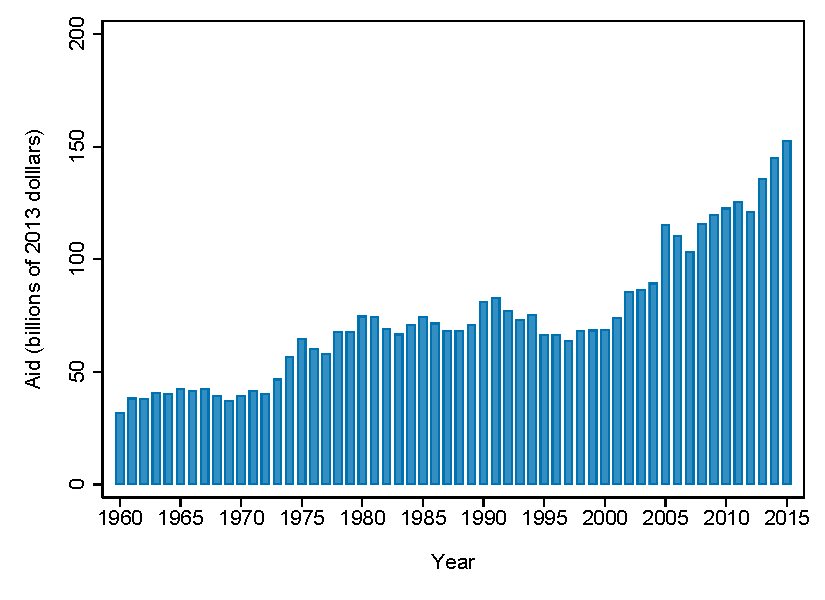
\includegraphics[width=7.2cm]{fig/aid-by-year.pdf} \\
		
		Between 1960 and 2015, developing countries received 4.15 trillion dollars in foreign aid 
\end{center}

\end{frame}


%%%%%%%%%%%%%%%%%%%%%%%%%%%%%%%%%%%%%%%%%%%%%%%%%%%%%%%%%%%%%%%%%%%%%

\begin{frame}{Why Does Aid Exist?}

\begin{center}
	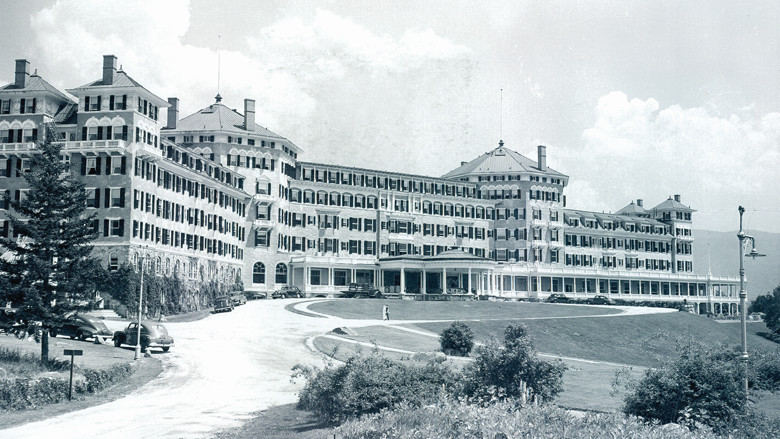
\includegraphics[height=3.2cm]{photos/bretton-woods-1944-WB-photo.jpg} 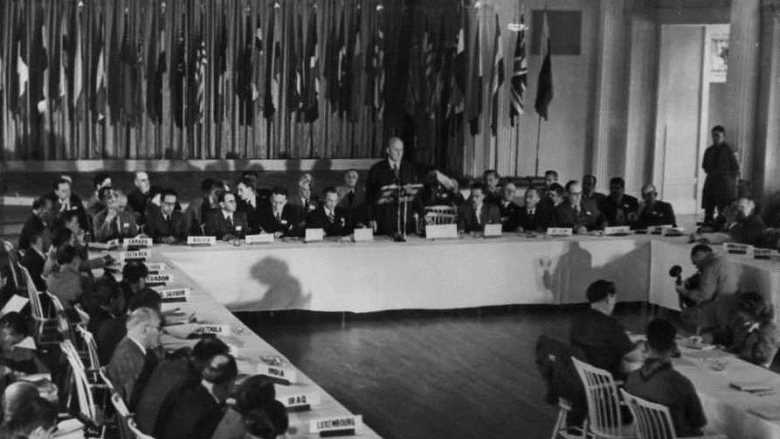
\includegraphics[height=3.2cm]{photos/BW-conf-hall-1944-WB-photo.jpg} \\
	\textcolor{gray}{\tiny{photos:  World Bank}}
	
	\medskip
	\medskip
	
	Aid is intended to reduce poverty and promote growth in ``less-developed'' countries \\
	(though this is not the only reason countries spend money on foreign aid)
\end{center}

\end{frame}

% Photos of the Bretton Woods Monetary Conference in 1944, in case that wasn't obvious


%% I'VE COMMENTED OUT THE SLIDES USING PHOTOS FROM THE WORLD BANK HISTORICAL PHOTO ARCHIVE
%% (TO KEEP THE FILE SIZE RELATIVELY SMALL)
%% ARCHIVE IS HERE:  https://archivesphotos.worldbank.org/en/about/archives/photo-gallery/photo-gallery-landing

%%%%%%%%%%%%%%%%%%%%%%%%%%%%%%%%%%%%%%%%%%%%%%%%%%%%%%%%%%%%%%%%%%%%%%
%
%\begin{frame}<handout:0>{What Was Aid Used For?}
%
%\begin{center}
%	\includegraphics[height=3.2cm]{photos/Kenyatta-Kibaki-McNamara-1973-WBG.jpeg} $\ \ $	\includegraphics[height=3.2cm]{photos/Kenya-road-1960-Ivan-Massar-WB.jpeg} \\
%	%\includegraphics[height=3.2cm]{photos/TZ-loan-signing-Tan-Zam-highway-1969-Edwin-Huffman-WB.jpeg} $\ \ $	%\includegraphics[height=3.2cm]{photos/TZ-road-near-Msata-1969-Per-Gunvall-WB.jpg} \\
%	\textcolor{gray}{\tiny{photos:  World Bank}}
%	
%	\medskip
%	\medskip
%	
%	In 1960, Kenya borrowed 5.6 million (not inflation-adjusted) dollars for road construction
%\end{center}
%
%\end{frame}
%
%
%%%%%%%%%%%%%%%%%%%%%%%%%%%%%%%%%%%%%%%%%%%%%%%%%%%%%%%%%%%%%%%%%%%%%%
%
%\begin{frame}<handout:0>{What Was Aid Used For?}
%
%\begin{center}
%	%\includegraphics[height=3.2cm]{photos/Kenyatta-Kibaki-McNamara-1973-WBG.jpeg} $\ \ $	%\includegraphics[height=3.2cm]{photos/Kenya-road-1960-Ivan-Massar-WB.jpeg} \\
%	\includegraphics[height=3.2cm]{photos/TZ-loan-signing-Tan-Zam-highway-1969-Edwin-Huffman-WB.jpeg} $\ \ $	\includegraphics[height=3.2cm]{photos/TZ-road-near-Msata-1969-Per-Gunvall-WB.jpg} \\
%	
%	\textcolor{gray}{\tiny{photos:  World Bank}}
%
%\medskip
%\medskip
%
%Tanzania also took out loans to build roads, as well as other infrastructure projects
%
%\end{center}
%
%\end{frame}
%
%
%%%%%%%%%%%%%%%%%%%%%%%%%%%%%%%%%%%%%%%%%%%%%%%%%%%%%%%%%%%%%%%%%%%%%%
%
%\begin{frame}<handout:0>{What Was Aid Used For?}
%
%\begin{center}
%	%\includegraphics[height=3.2cm]{photos/Kenyatta-Kibaki-McNamara-1973-WBG.jpeg} $\ \ $	%\includegraphics[height=3.2cm]{photos/Kenya-road-1960-Ivan-Massar-WB.jpeg} \\
%	\includegraphics[height=3.2cm]{photos/volta-dam-site-George-Gerster-1963.jpeg} $\ \ $	\includegraphics[height=3.2cm]{photos/volta-dam-pamela-johnson-1968.jpeg} \\
%	
%	\textcolor{gray}{\tiny{photos:  Pamela Johnson and George Gerster, World Bank}}
%	
%	\medskip
%	\medskip
%	
%	The World Bank loaned Ghana 47 million US dollars to build the Volta River Dam
%	
%\end{center}
%
%\end{frame}
%
%
%%%%%%%%%%%%%%%%%%%%%%%%%%%%%%%%%%%%%%%%%%%%%%%%%%%%%%%%%%%%%%%%%%%%%%
%
%\begin{frame}<handout:0>{What Was Aid Used For?}
%
%\begin{center}
%	%\includegraphics[height=3.2cm]{photos/Kenyatta-Kibaki-McNamara-1973-WBG.jpeg} $\ \ $	%\includegraphics[height=3.2cm]{photos/Kenya-road-1960-Ivan-Massar-WB.jpeg} \\
%	\includegraphics[height=3.2cm]{photos/IC-teacher-Hilda-Bijur-1972.jpg} $\ \ $	\includegraphics[height=3.2cm]{photos/IC-children-Hilda-Bijur-1972.jpg} \\
%	
%	\textcolor{gray}{\tiny{photos:  Hilda Bijur, World Bank}}
%	
%	\medskip
%	\medskip
%	
%	By the 1970s, World Bank lending more focused on ``basic needs'' rather than industrialization
%	
%\end{center}
%
%\end{frame}
%
%
%%%%%%%%%%%%%%%%%%%%%%%%%%%%%%%%%%%%%%%%%%%%%%%%%%%%%%%%%%%%%%%%%%%%%%
%
%\begin{frame}<handout:0>{What Was Aid Used For?}
%
%\begin{center}
%	%\includegraphics[height=3.2cm]{photos/Kenyatta-Kibaki-McNamara-1973-WBG.jpeg} $\ \ $	%\includegraphics[height=3.2cm]{photos/Kenya-road-1960-Ivan-Massar-WB.jpeg} \\
%	\includegraphics[height=3.2cm]{photos/Senegal-mcnamara-senghor-edwin-huffman-1971.jpg} $\ \ $	\includegraphics[height=3.2cm]{photos/Senegal-rice-project-Ray-Witlin-1974.jpg} \\
%	
%	\textcolor{gray}{\tiny{photos:  Edwin Huffman and Ray Witlin, World Bank}}
%	
%	\medskip
%	\medskip
%	
%	Senegal borrowed more than 10 million dollars and received more than 7 million dollars in aid to fund a series of agricultural modernization projects in the 1970s
%	
%\end{center}
%
%\end{frame}



%%%%%%%%%%%%%%%%%%%%%%%%%%%%%%%%%%%%%%%%%%%%%%%%%%%%%%%%%%%%%%%%%%%%%

\begin{frame}{A 90-Second History of Foreign Aid}


\medskip
\textbf{1960s:}  the \textbf{Big Push} -- aid for infrastructure and industrialization

\medskip
\medskip
\textbf{1970s:}  after failure of the Big Push, lending shifts toward meeting \textbf{basic needs} 

\medskip
\medskip
\textbf{1980s:}  the debt crisis and \textbf{structural adjustment} lending 

\medskip
\medskip
\textbf{1990s:}  governance, NGOs, beginnings of the modern era (in foreign aid)

\medskip
\medskip
\textbf{Epilogue:}  Millennium Development Goals, Sustainable Development Goals


\end{frame}



%%%%%%%%%%%%%%%%%%%%%%%%%%%%%%%%%%%%%%%%%%%%%%%%%%%%%%%%%%%%%%%%%%%%%

\begin{frame}{Which Countries Received the Most Aid?}

\begin{center}
	\fbox{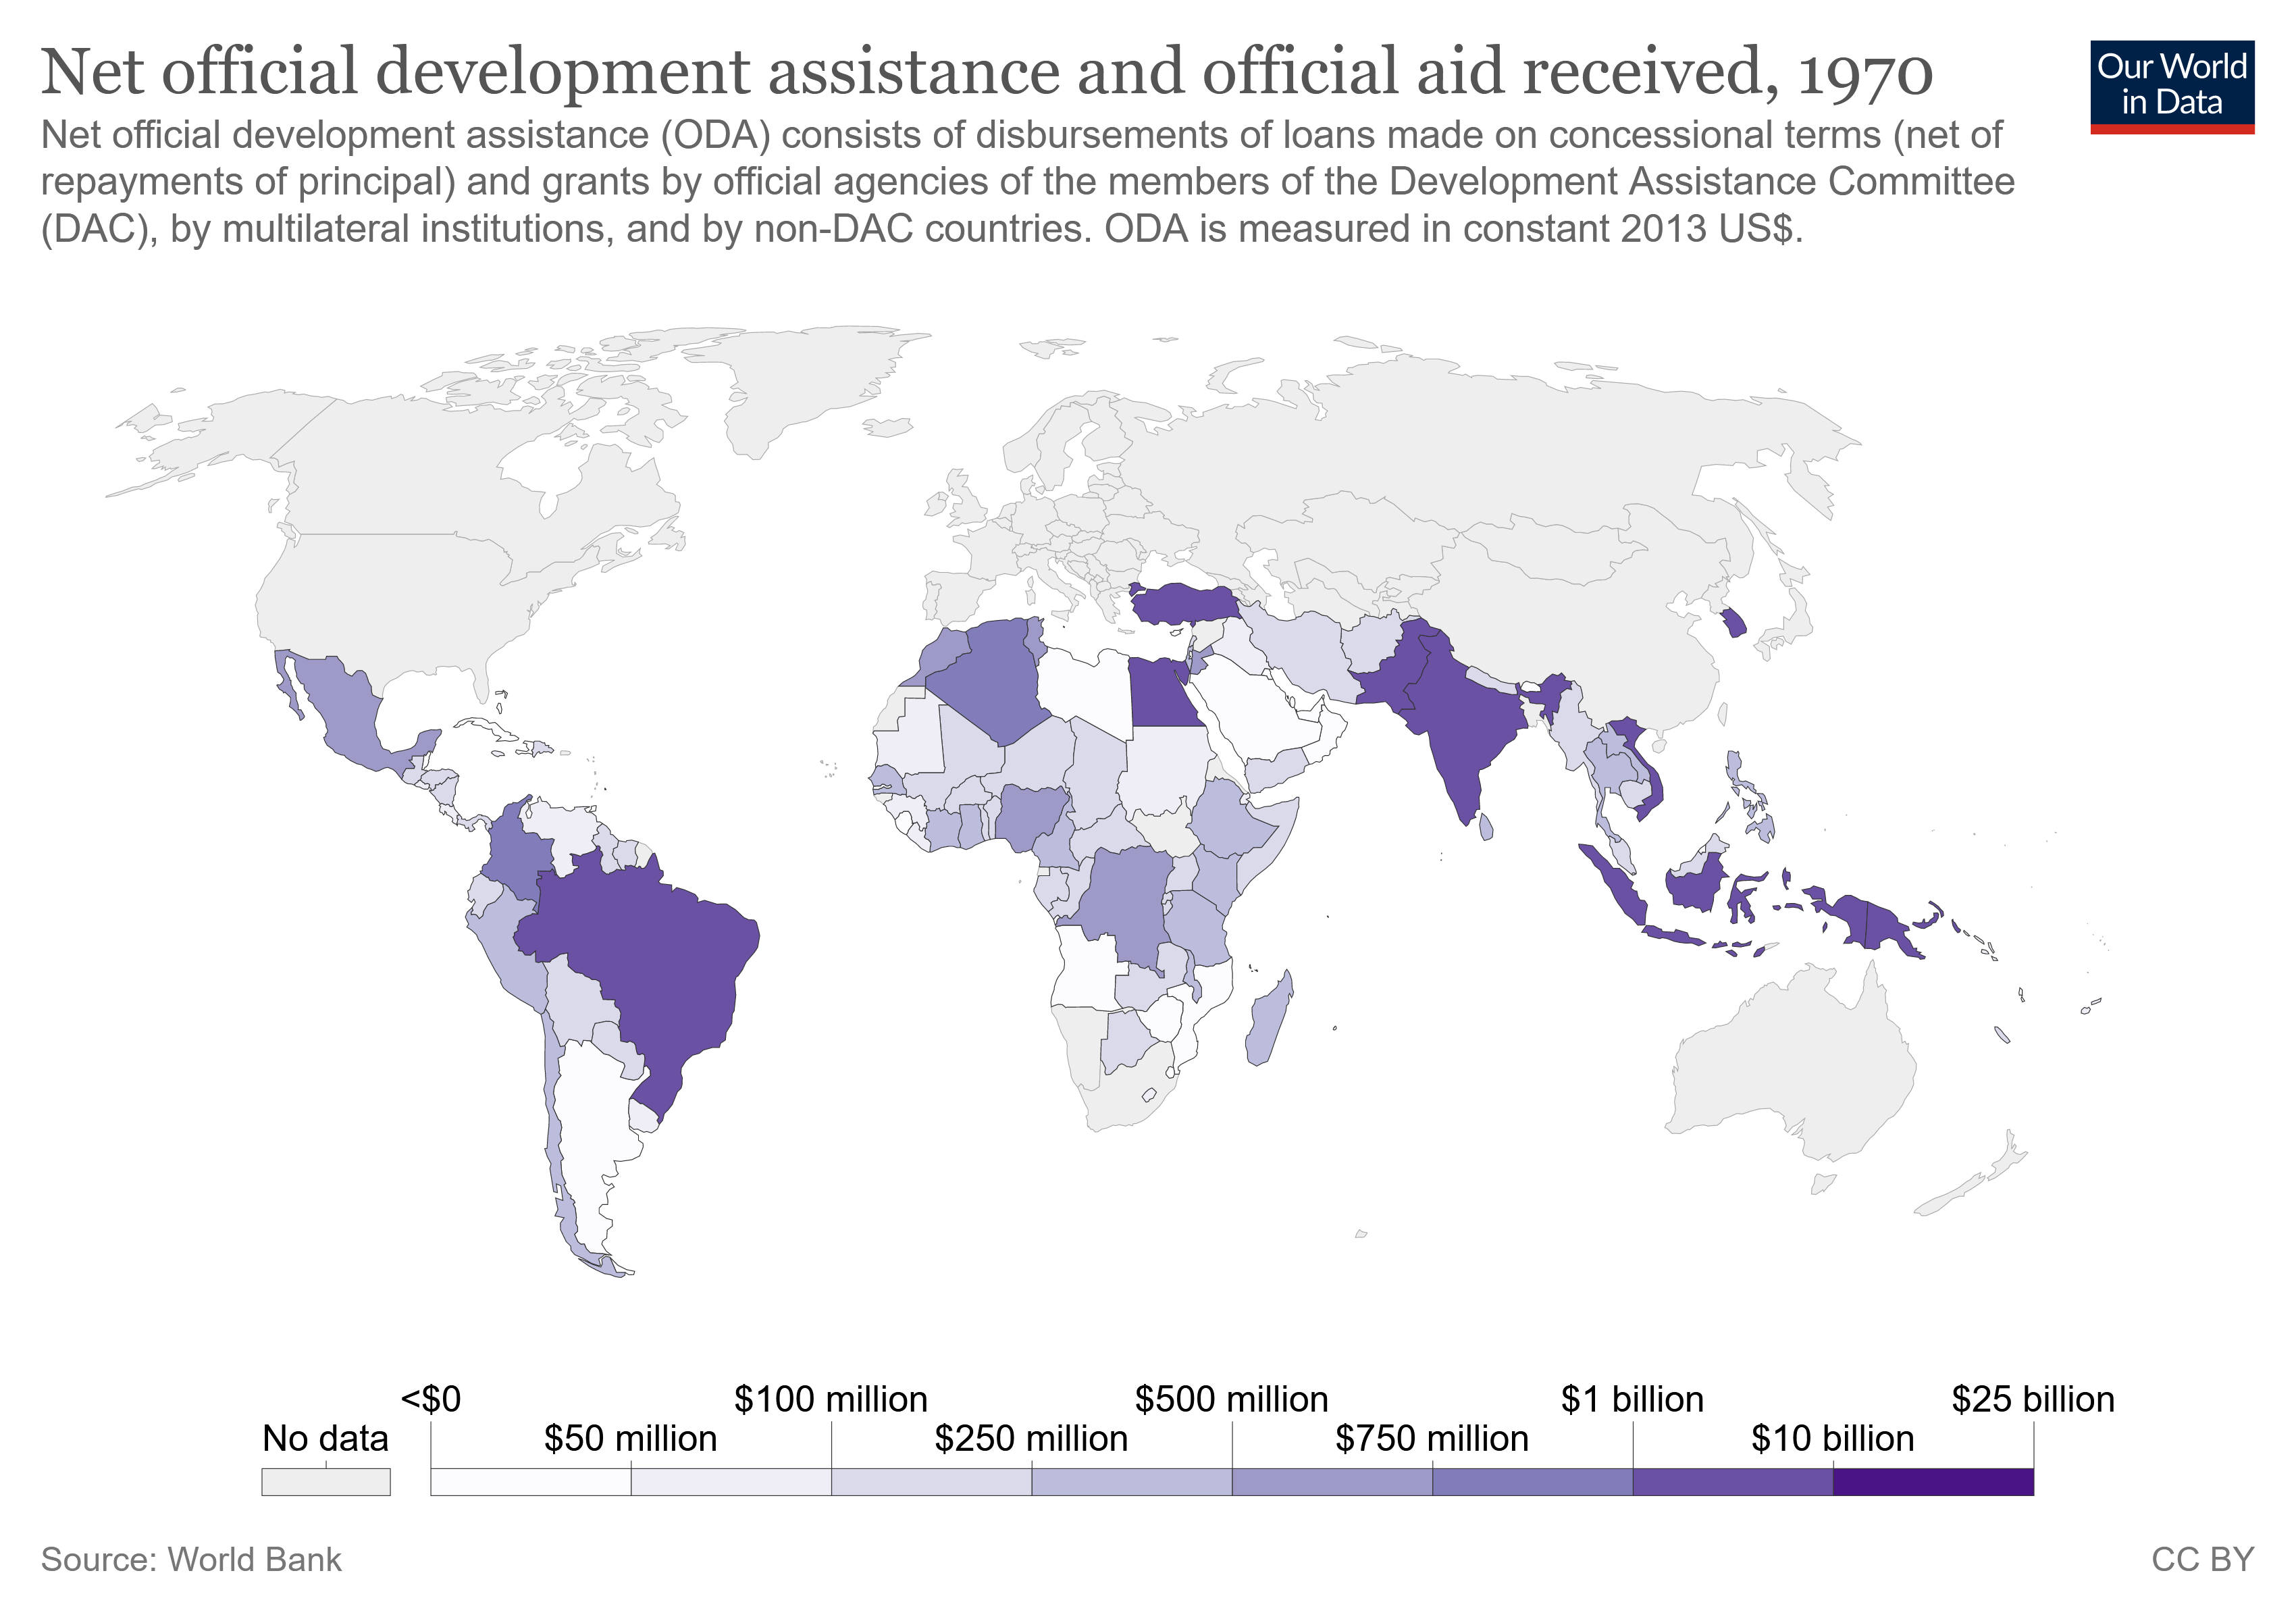
\includegraphics[height=3.2cm]{img/OWiD-aid-1970.png}} $\ \ $	\fbox{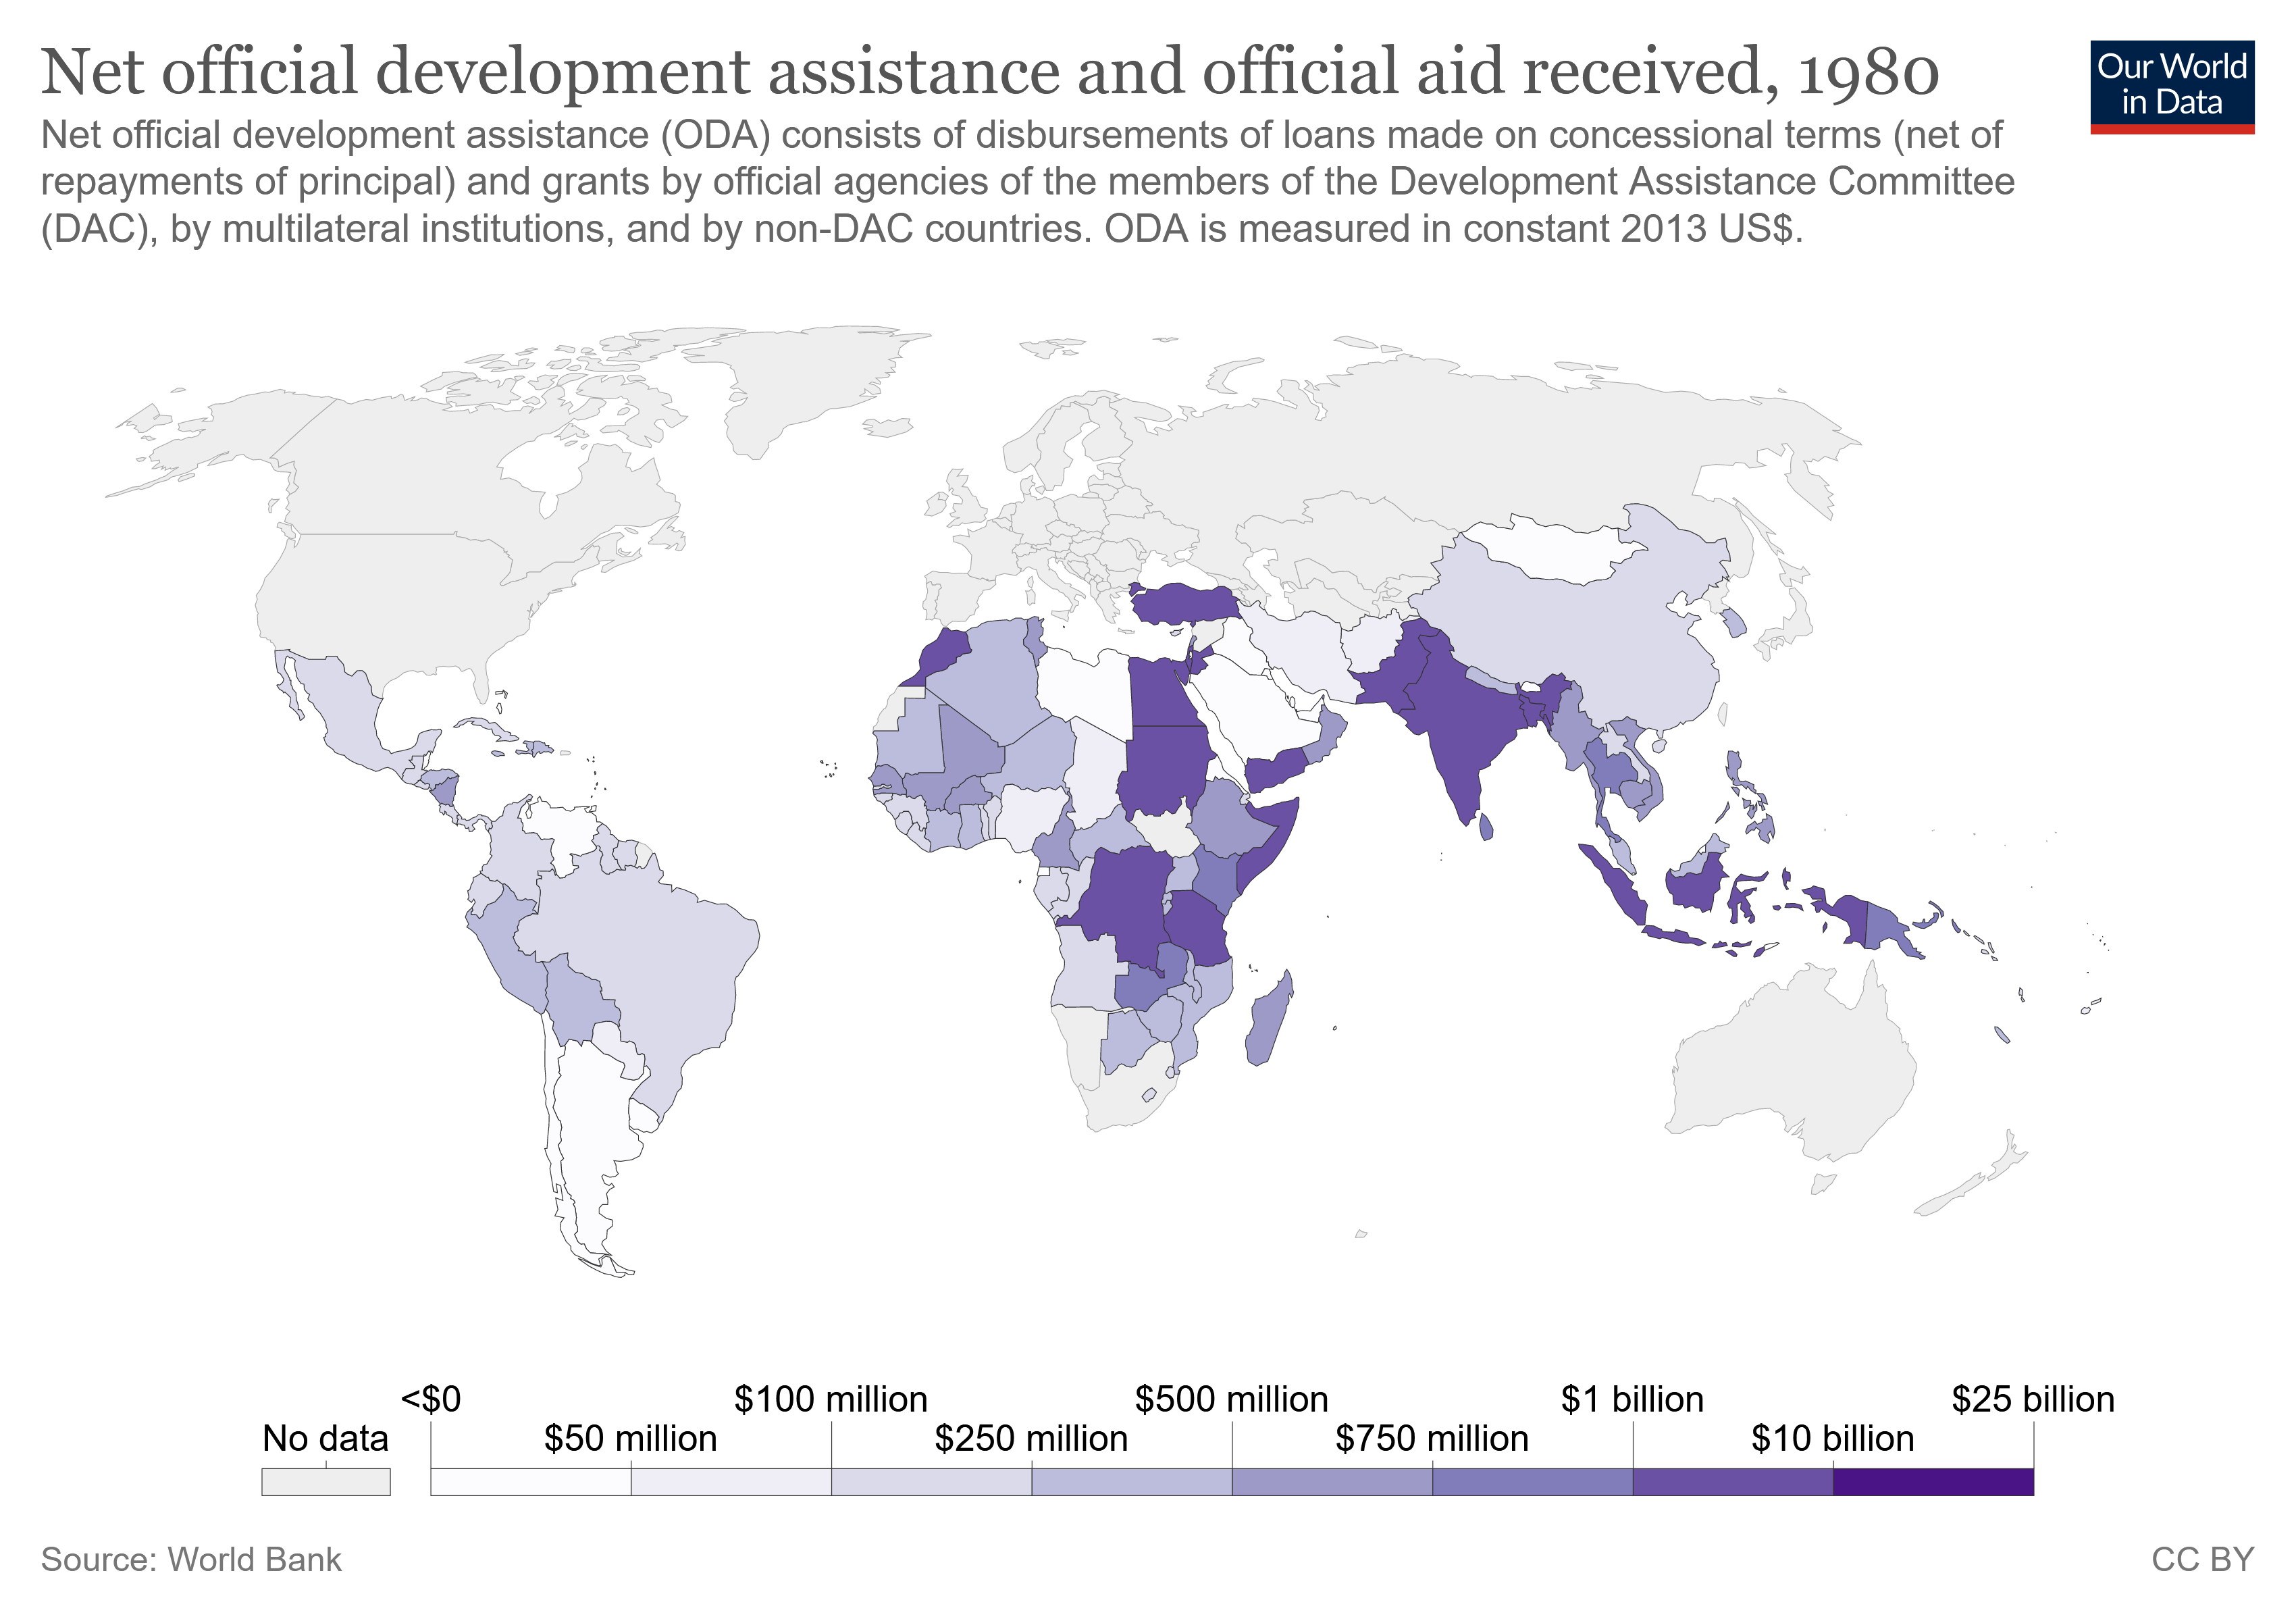
\includegraphics[height=3.2cm]{img/OWiD-aid-1980.png}} \\
		\fbox{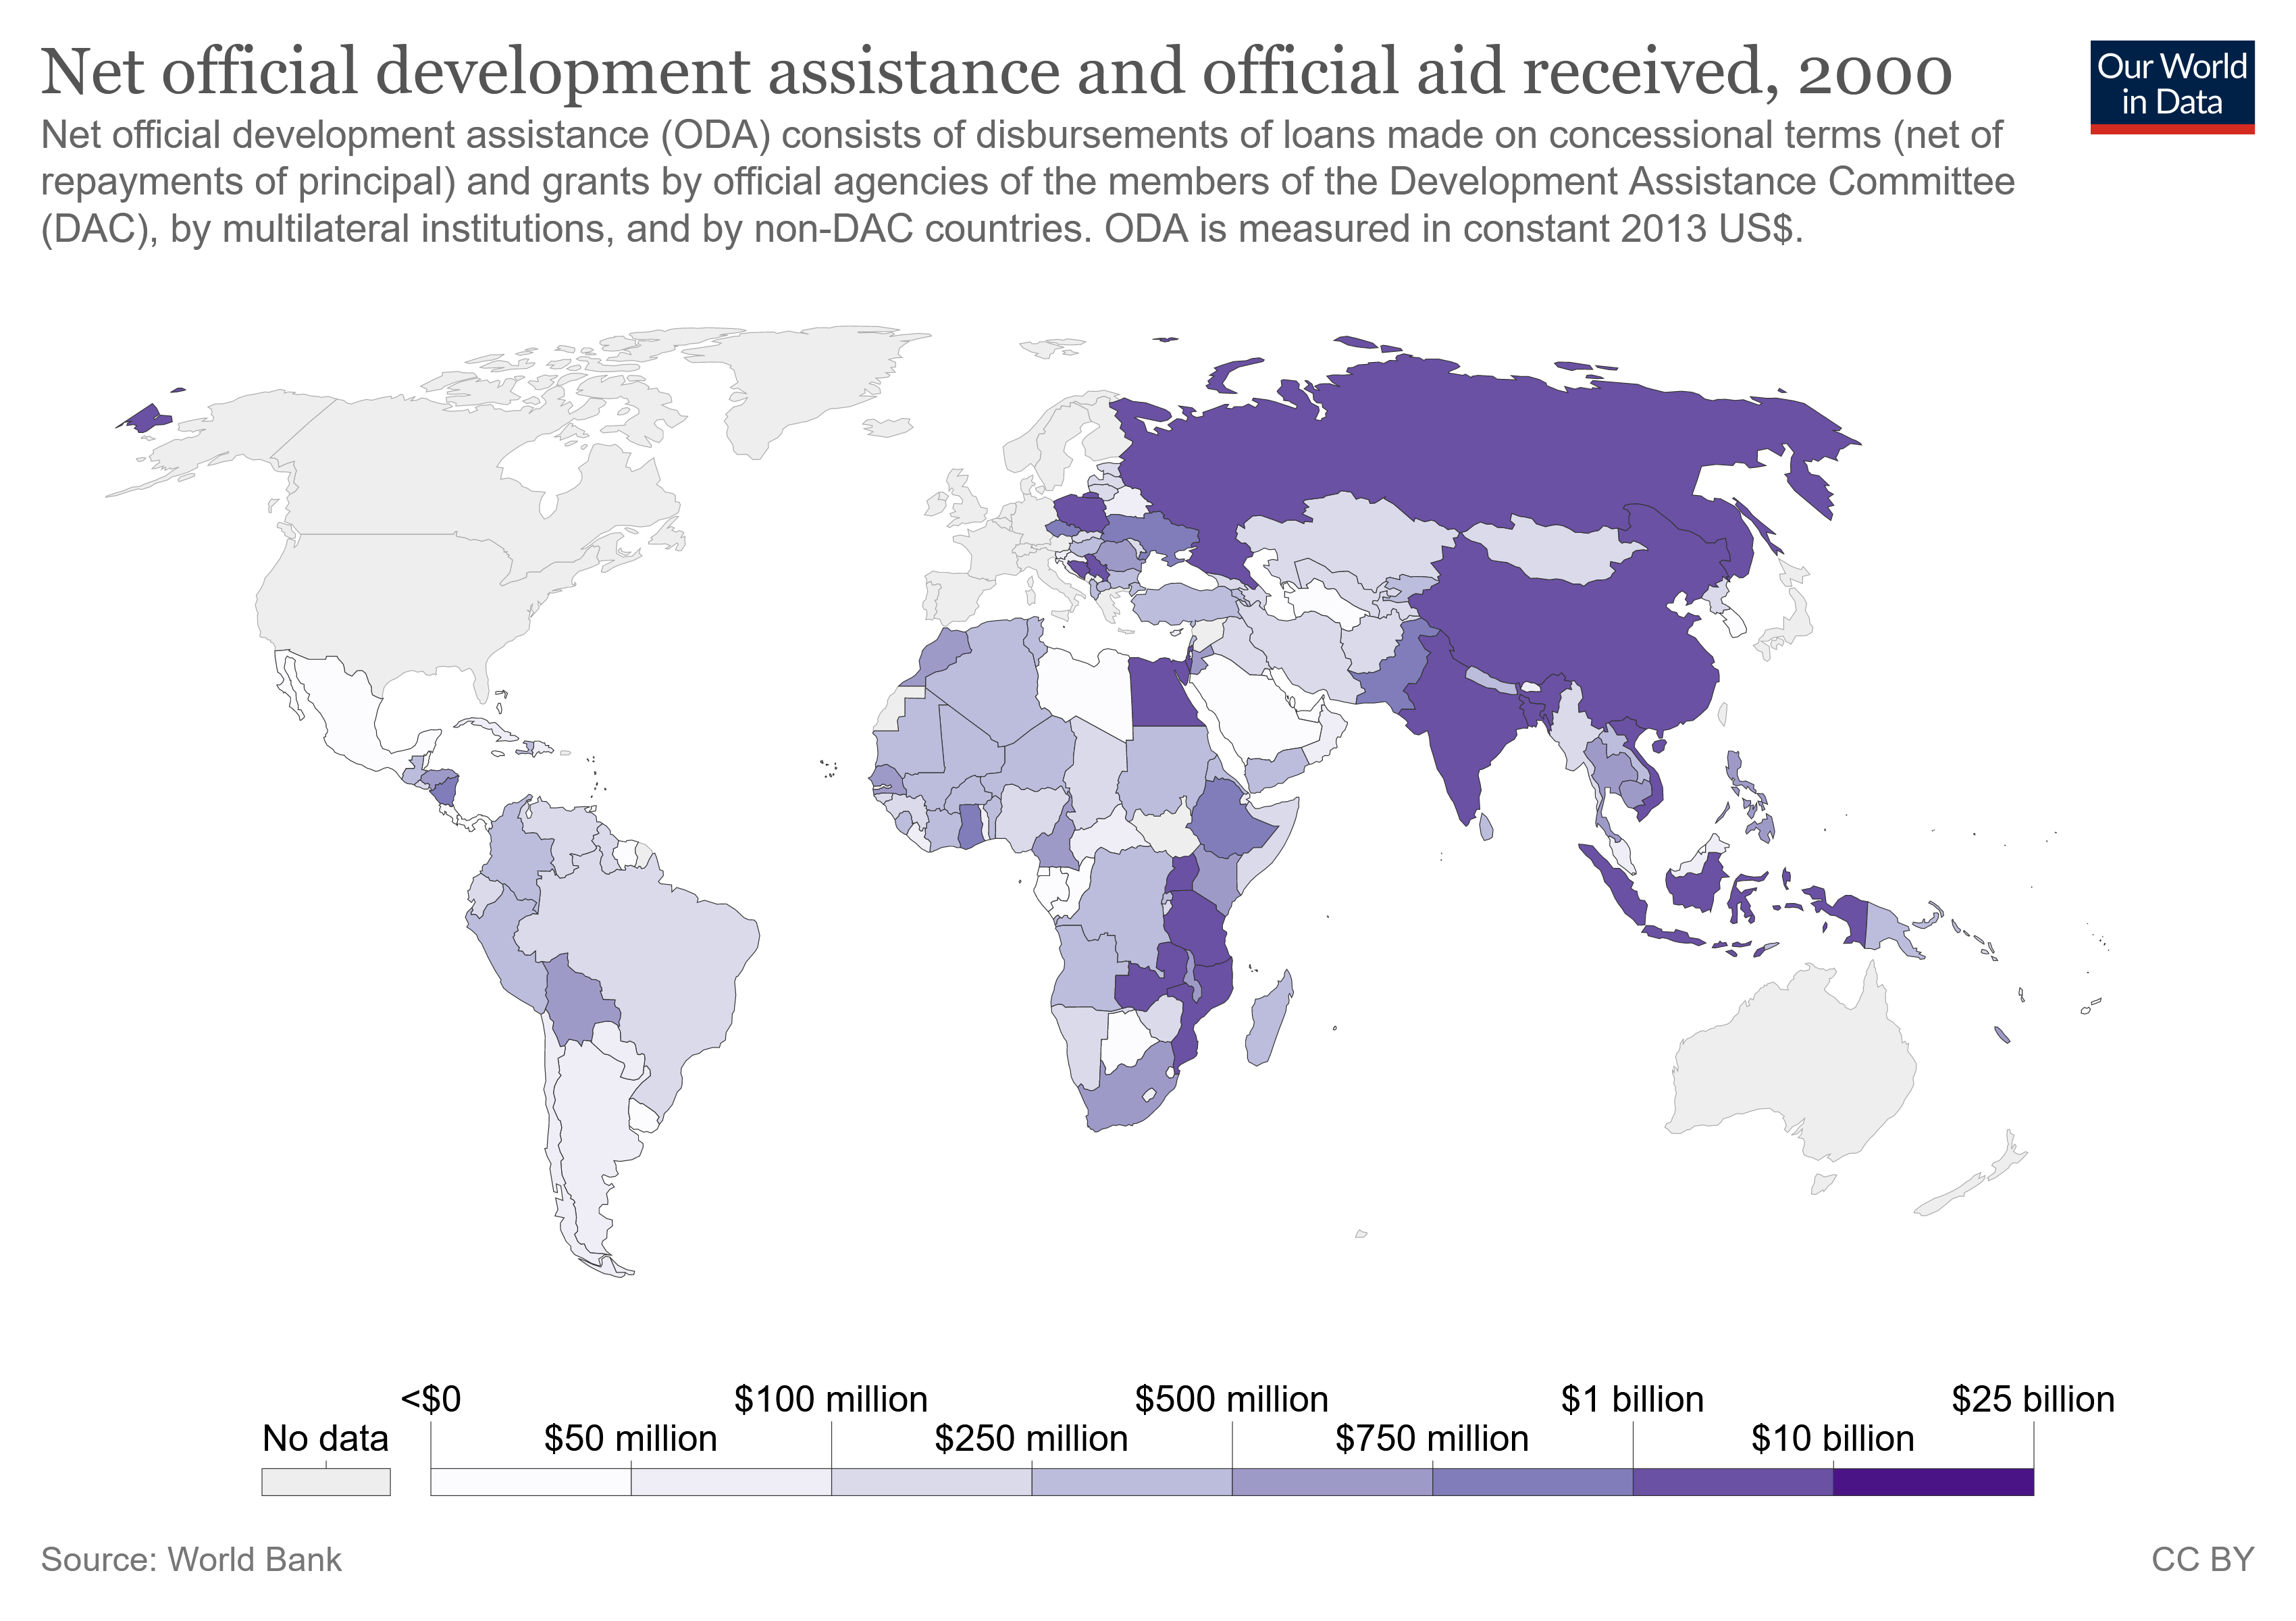
\includegraphics[height=3.2cm]{img/OWiD-aid-2000.png}} $\ \ $	\fbox{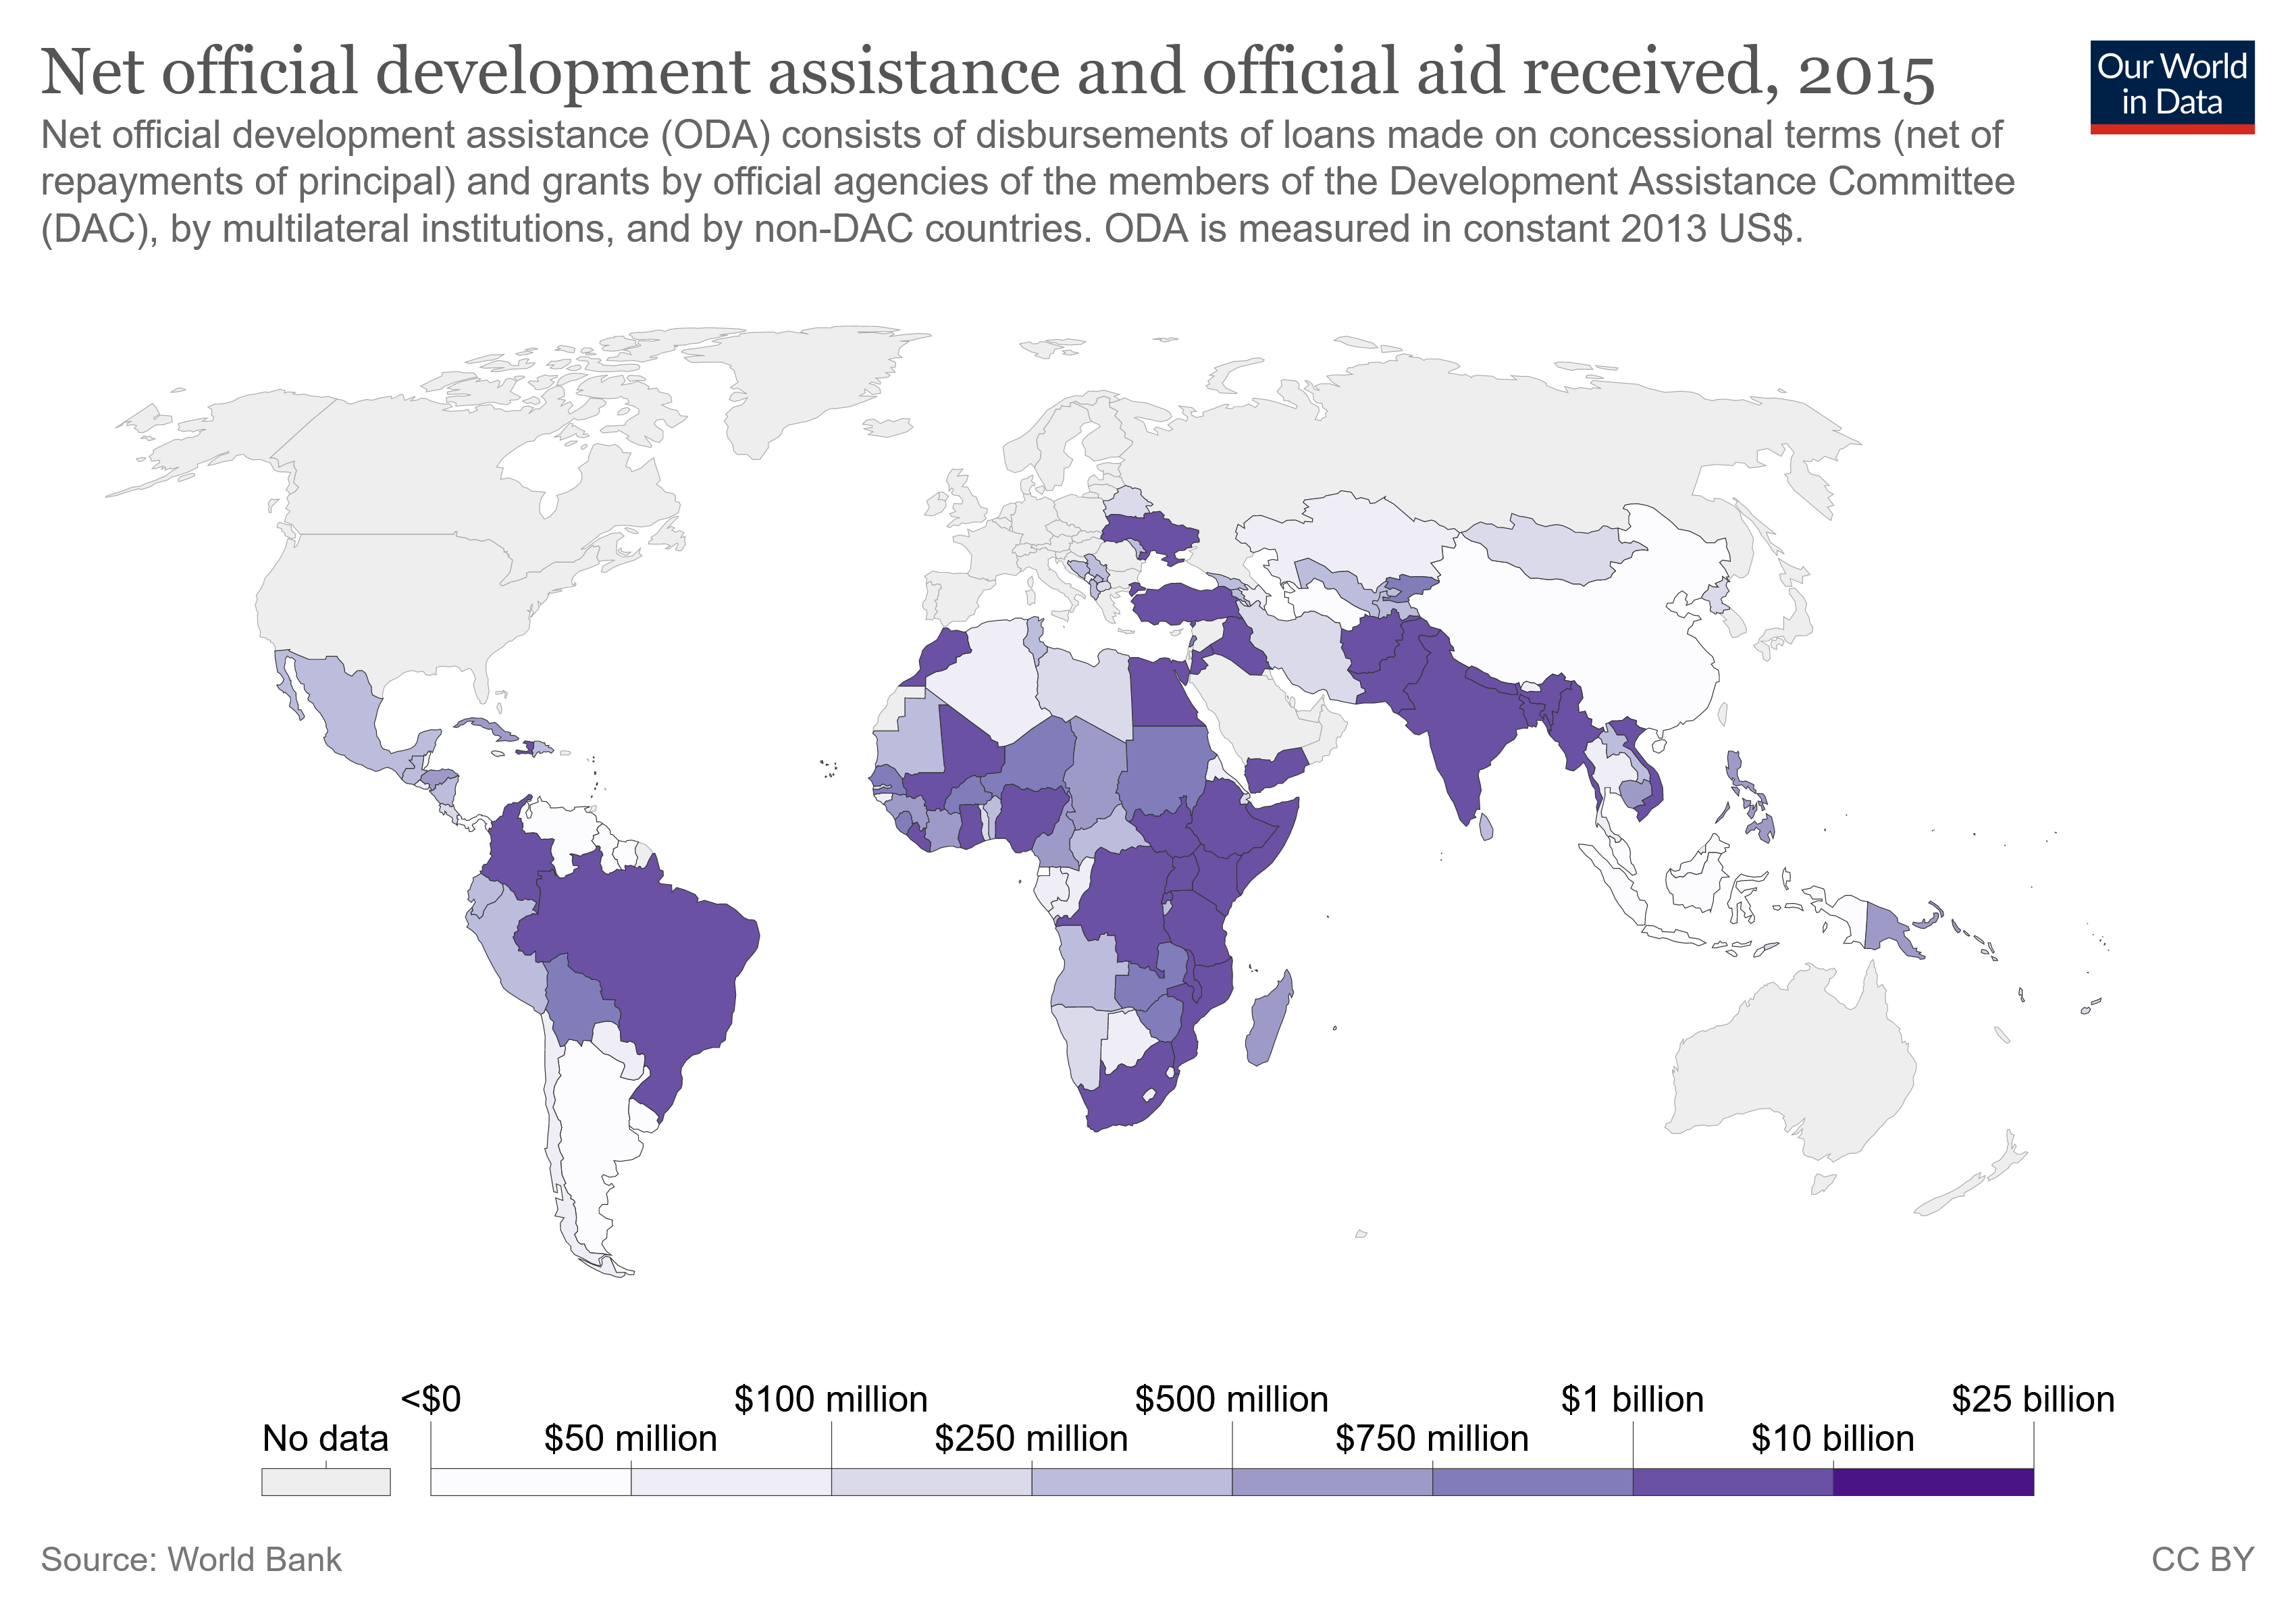
\includegraphics[height=3.2cm]{img/OWiD-aid-2015.png}} \\
	
%	Between 1960 and 2015, developing countries received 4.15 trillion dollars in foreign aid 
\end{center}

\end{frame}



%%%%%%%%%%%%%%%%%%%%%%%%%%%%%%%%%%%%%%%%%%%%%%%%%%%%%%%%%%%%%%%%%%%%%

\begin{frame}{Did Aid Lead to Better Development Outcomes?}

\begin{center}
	\fbox{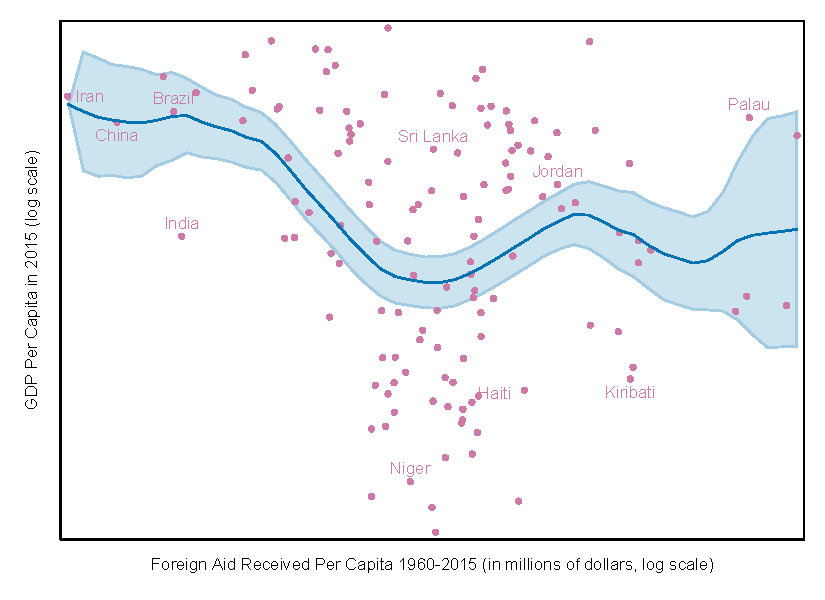
\includegraphics[height=4cm]{fig/aid-vs-gdp.pdf}} $\ \ $	\fbox{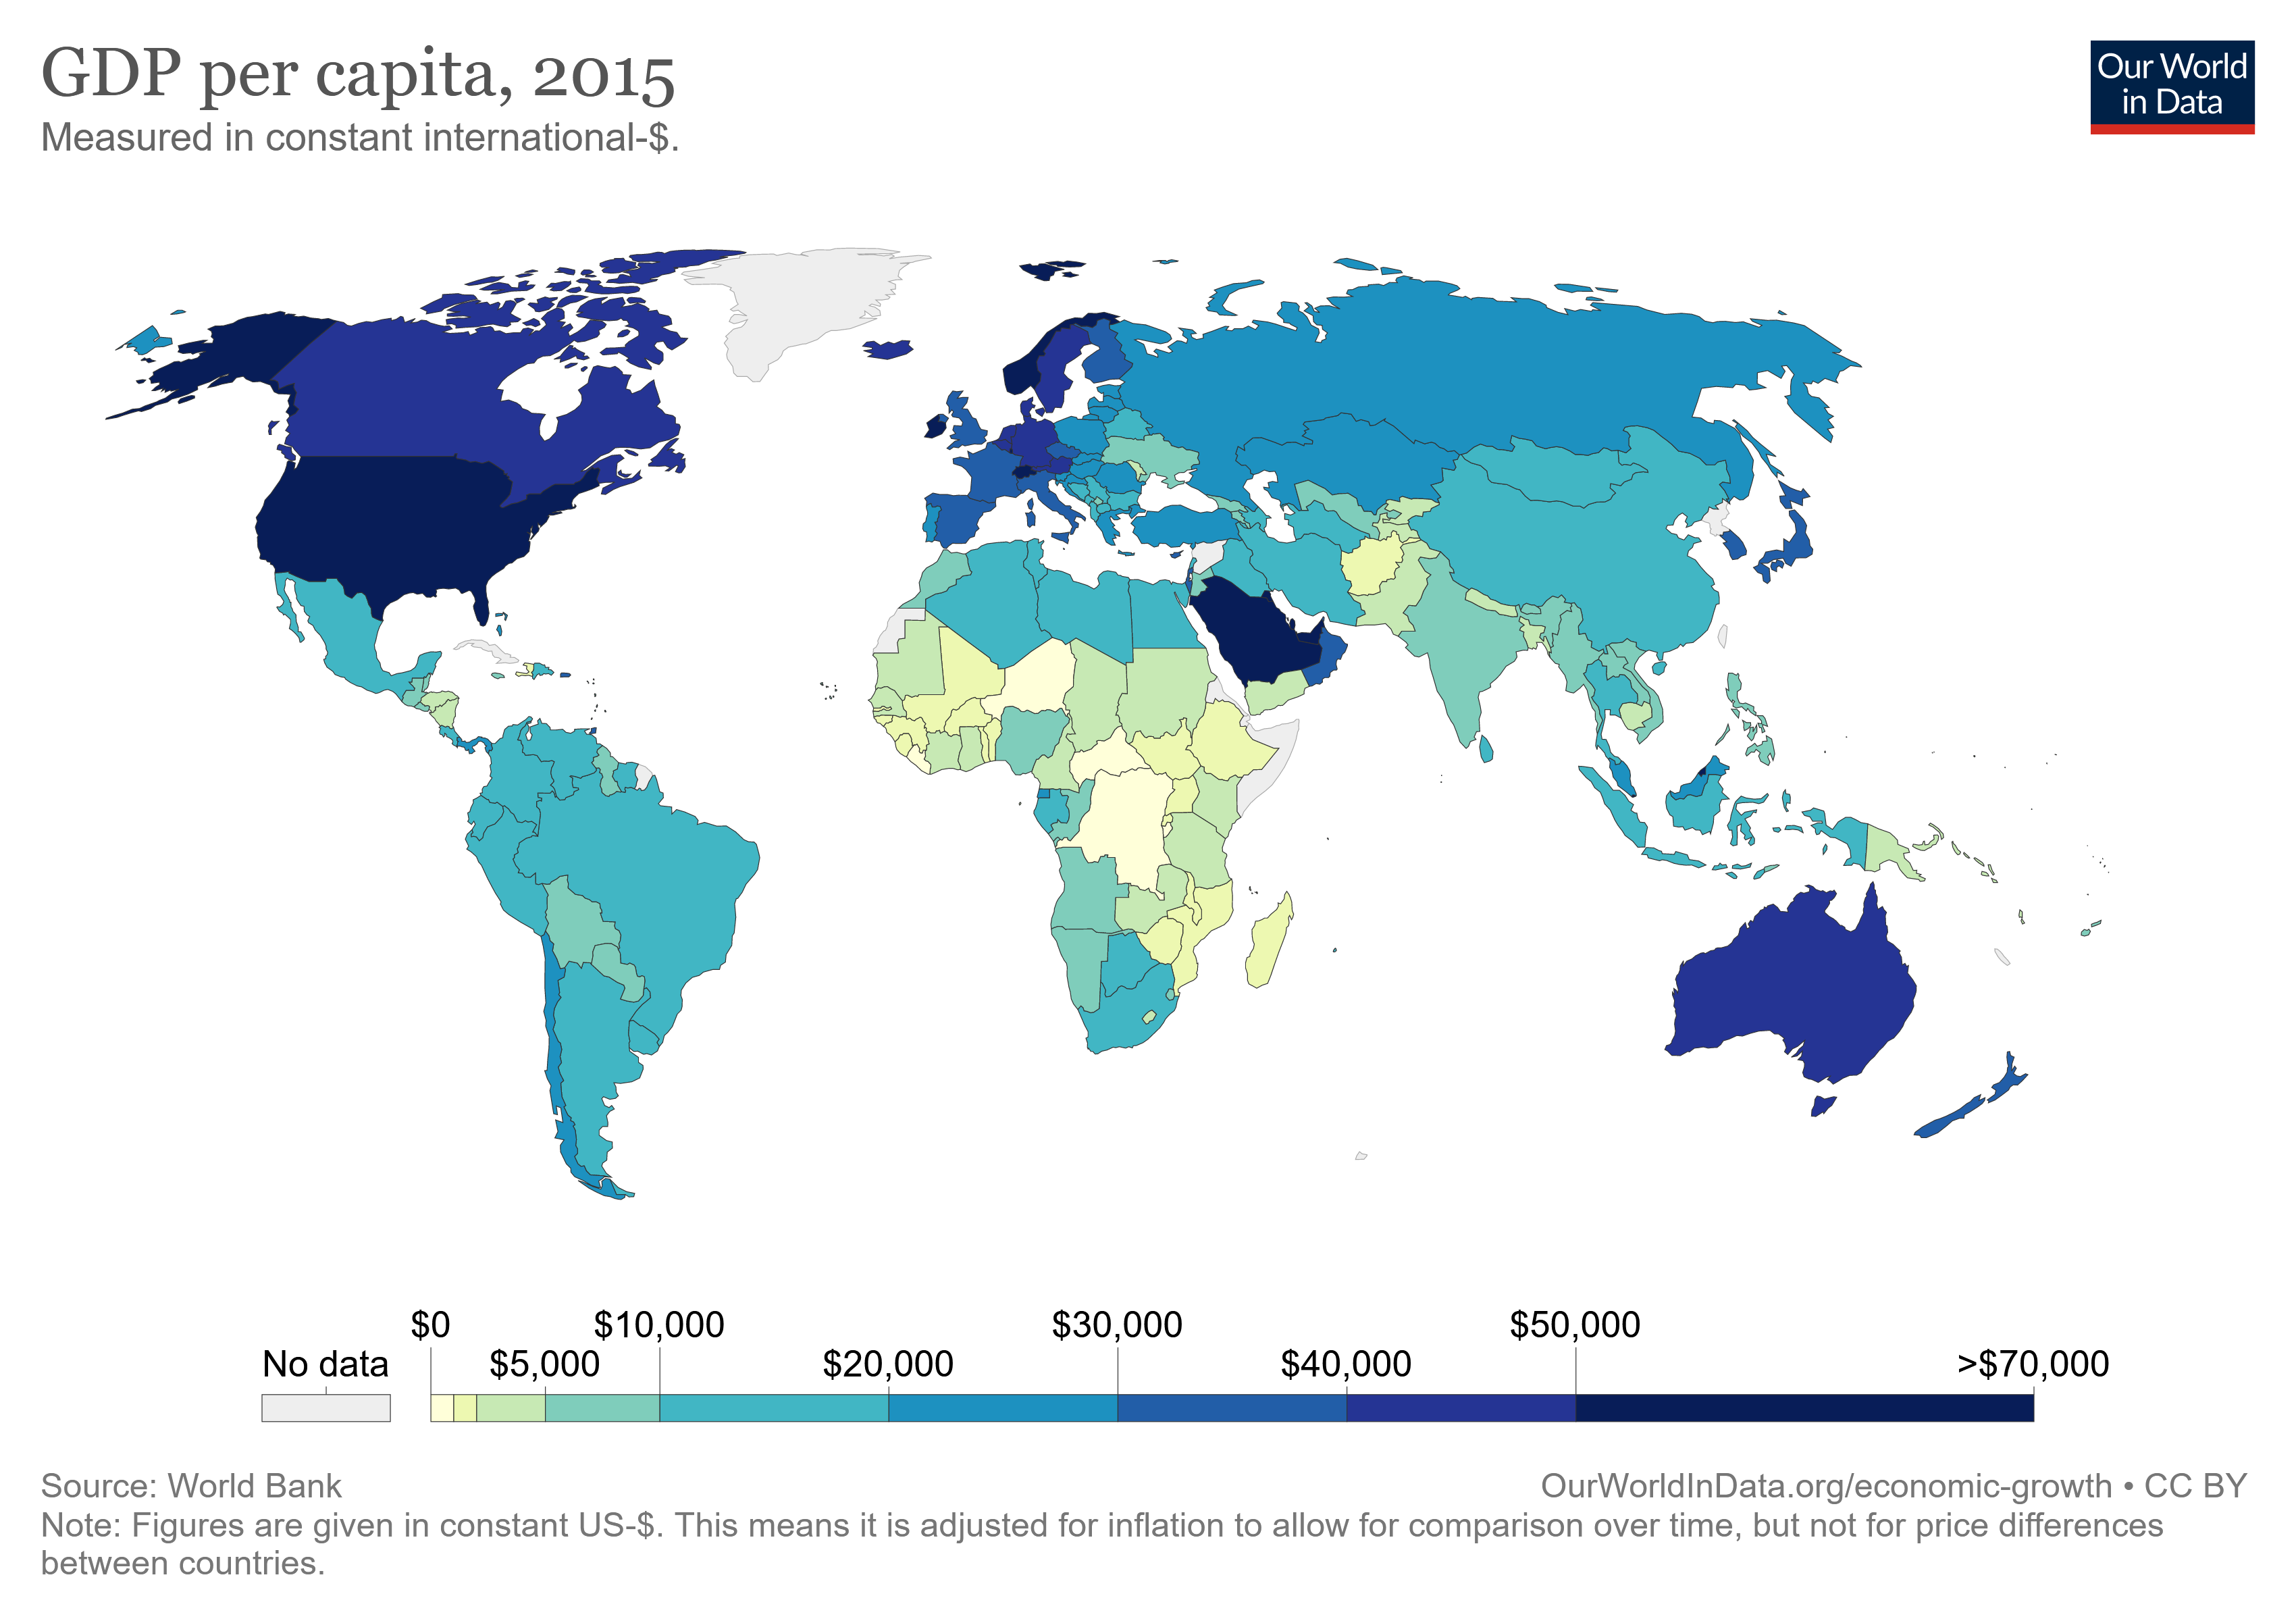
\includegraphics[height=4cm]{img/OWiD-gdp-per-capita.png}} \\
	
	\medskip
	\medskip
	
	Many countries that received substantial amounts of aid per capita are still very poor 
\end{center}

\end{frame}


%%%%%%%%%%%%%%%%%%%%%%%%%%%%%%%%%%%%%%%%%%%%%%%%%%%%%%%%%%%%%%%%%%%%%

\begin{frame}{Did Aid Lead to Better Development Outcomes?}

\begin{center}
	\fbox{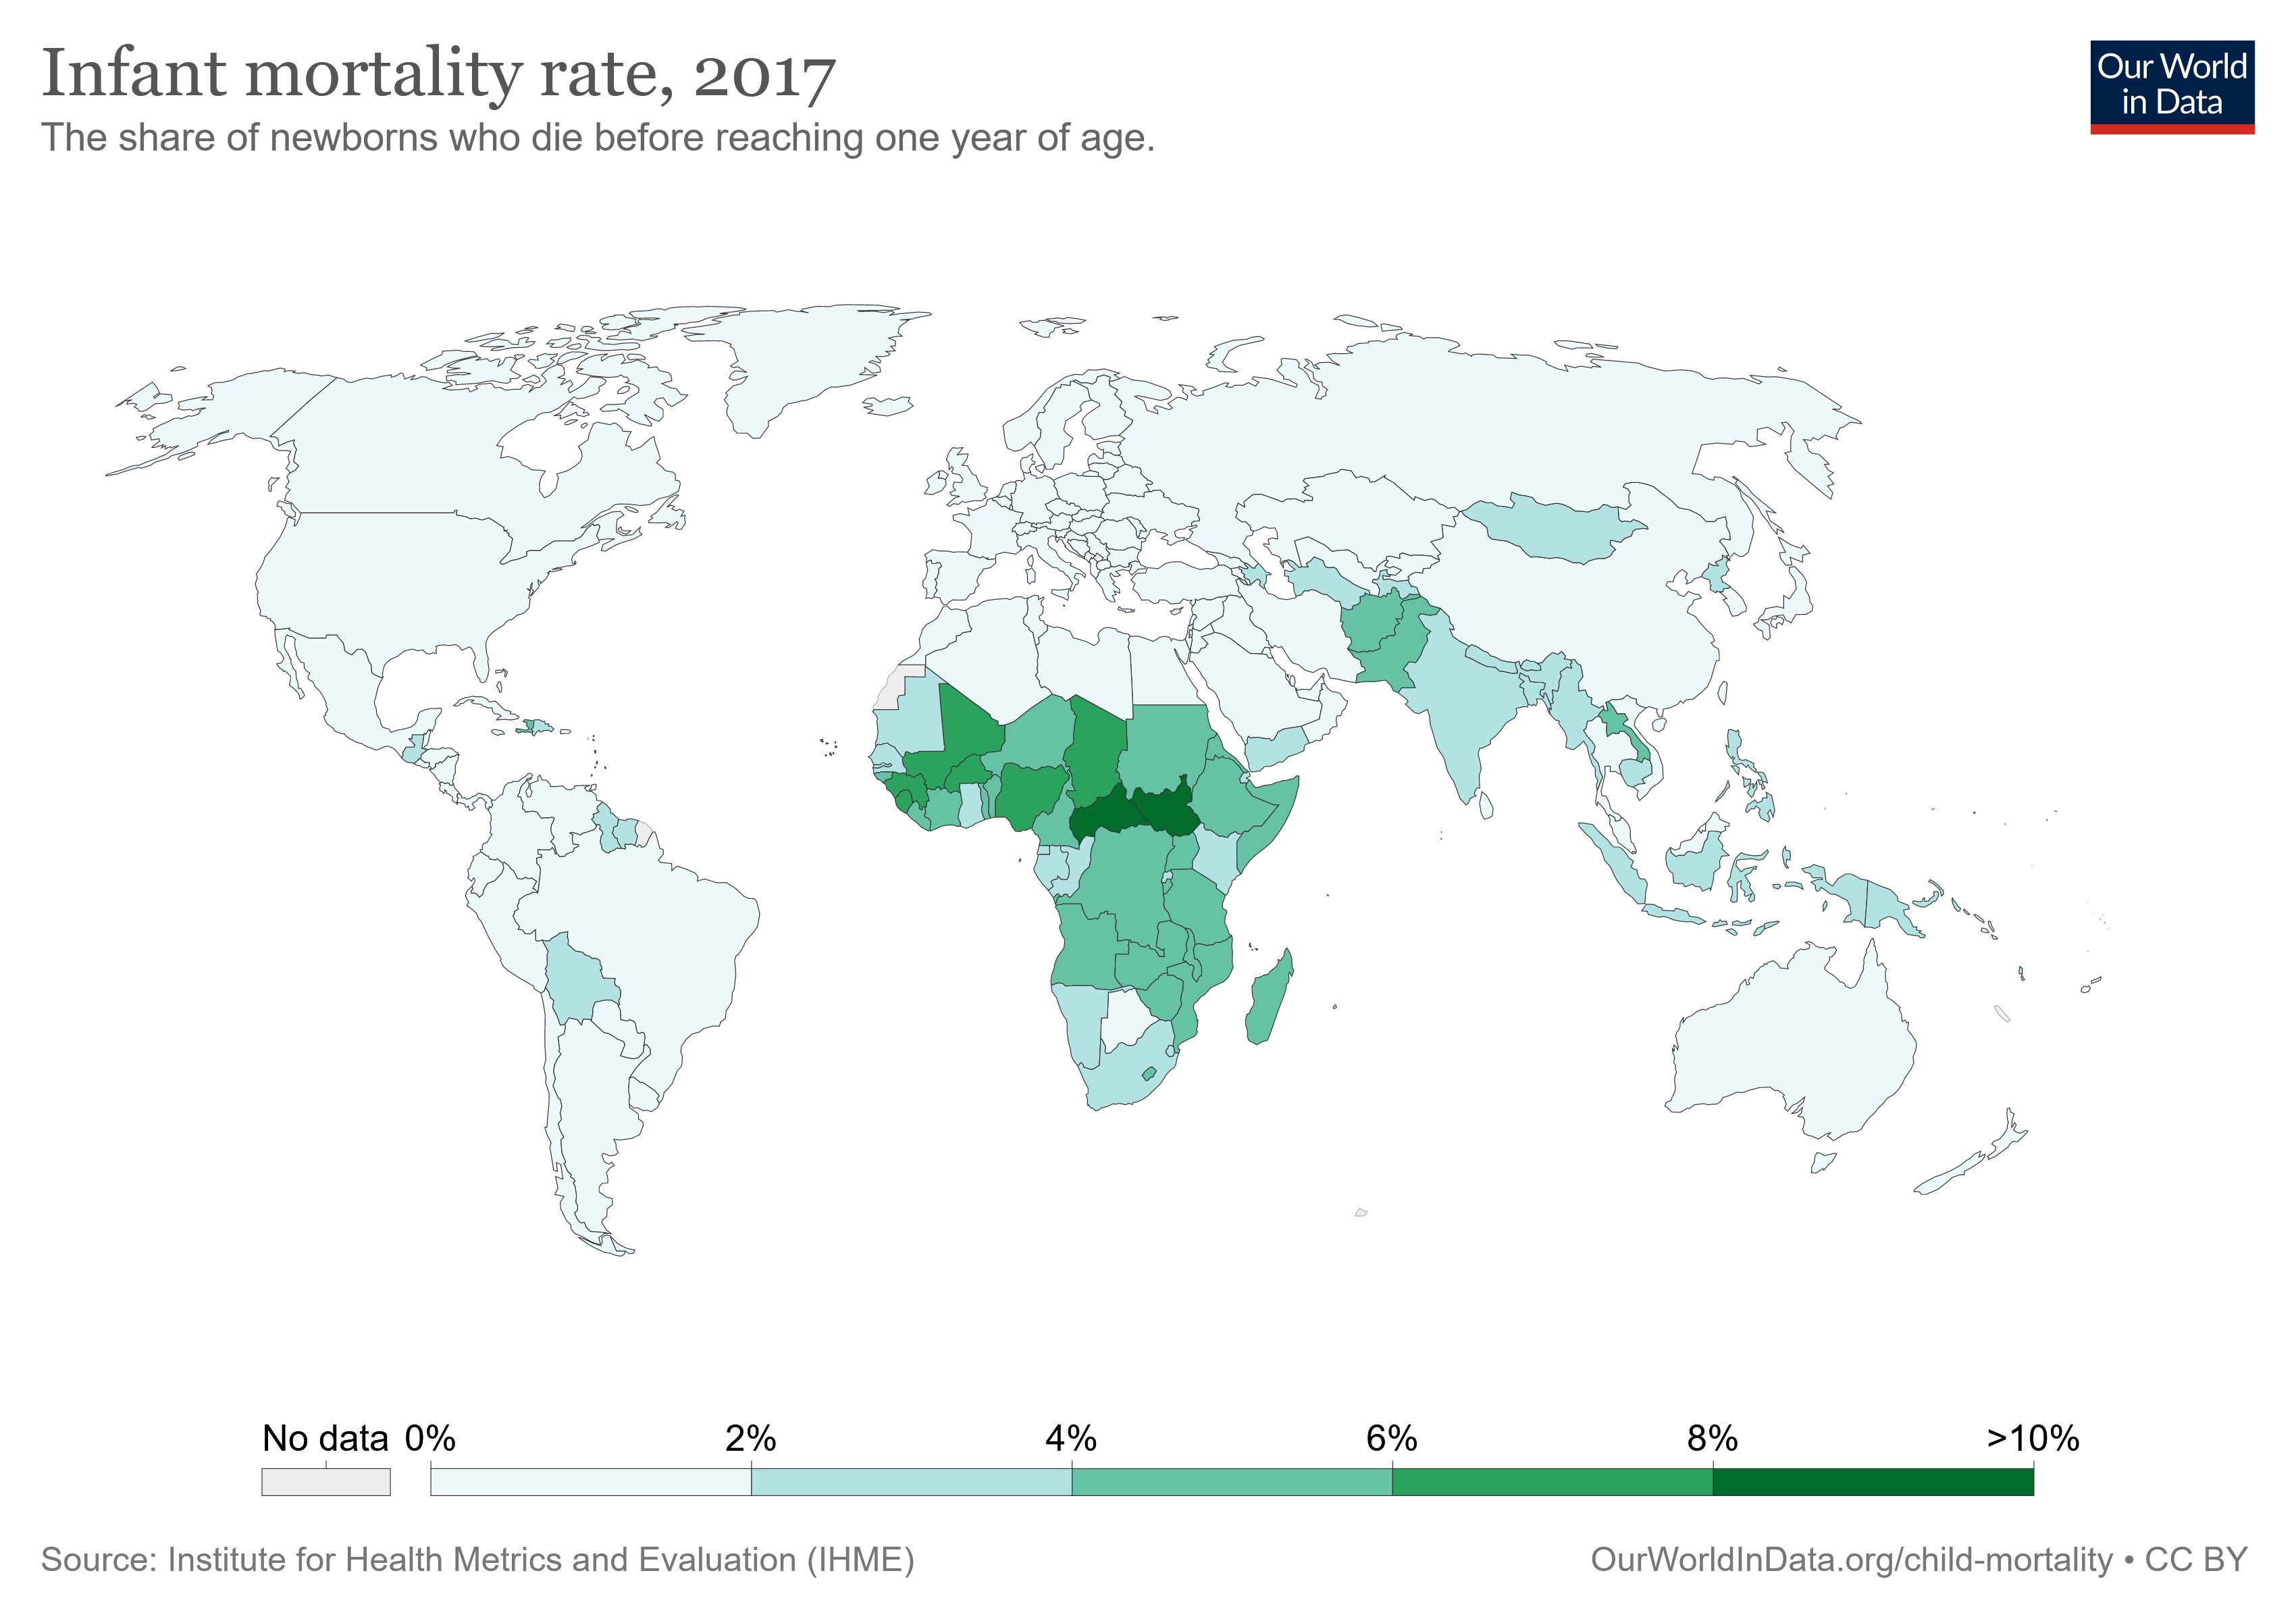
\includegraphics[height=3.2cm]{img/OWiD-infant-mortality-rate.png}} $\ \ $	\fbox{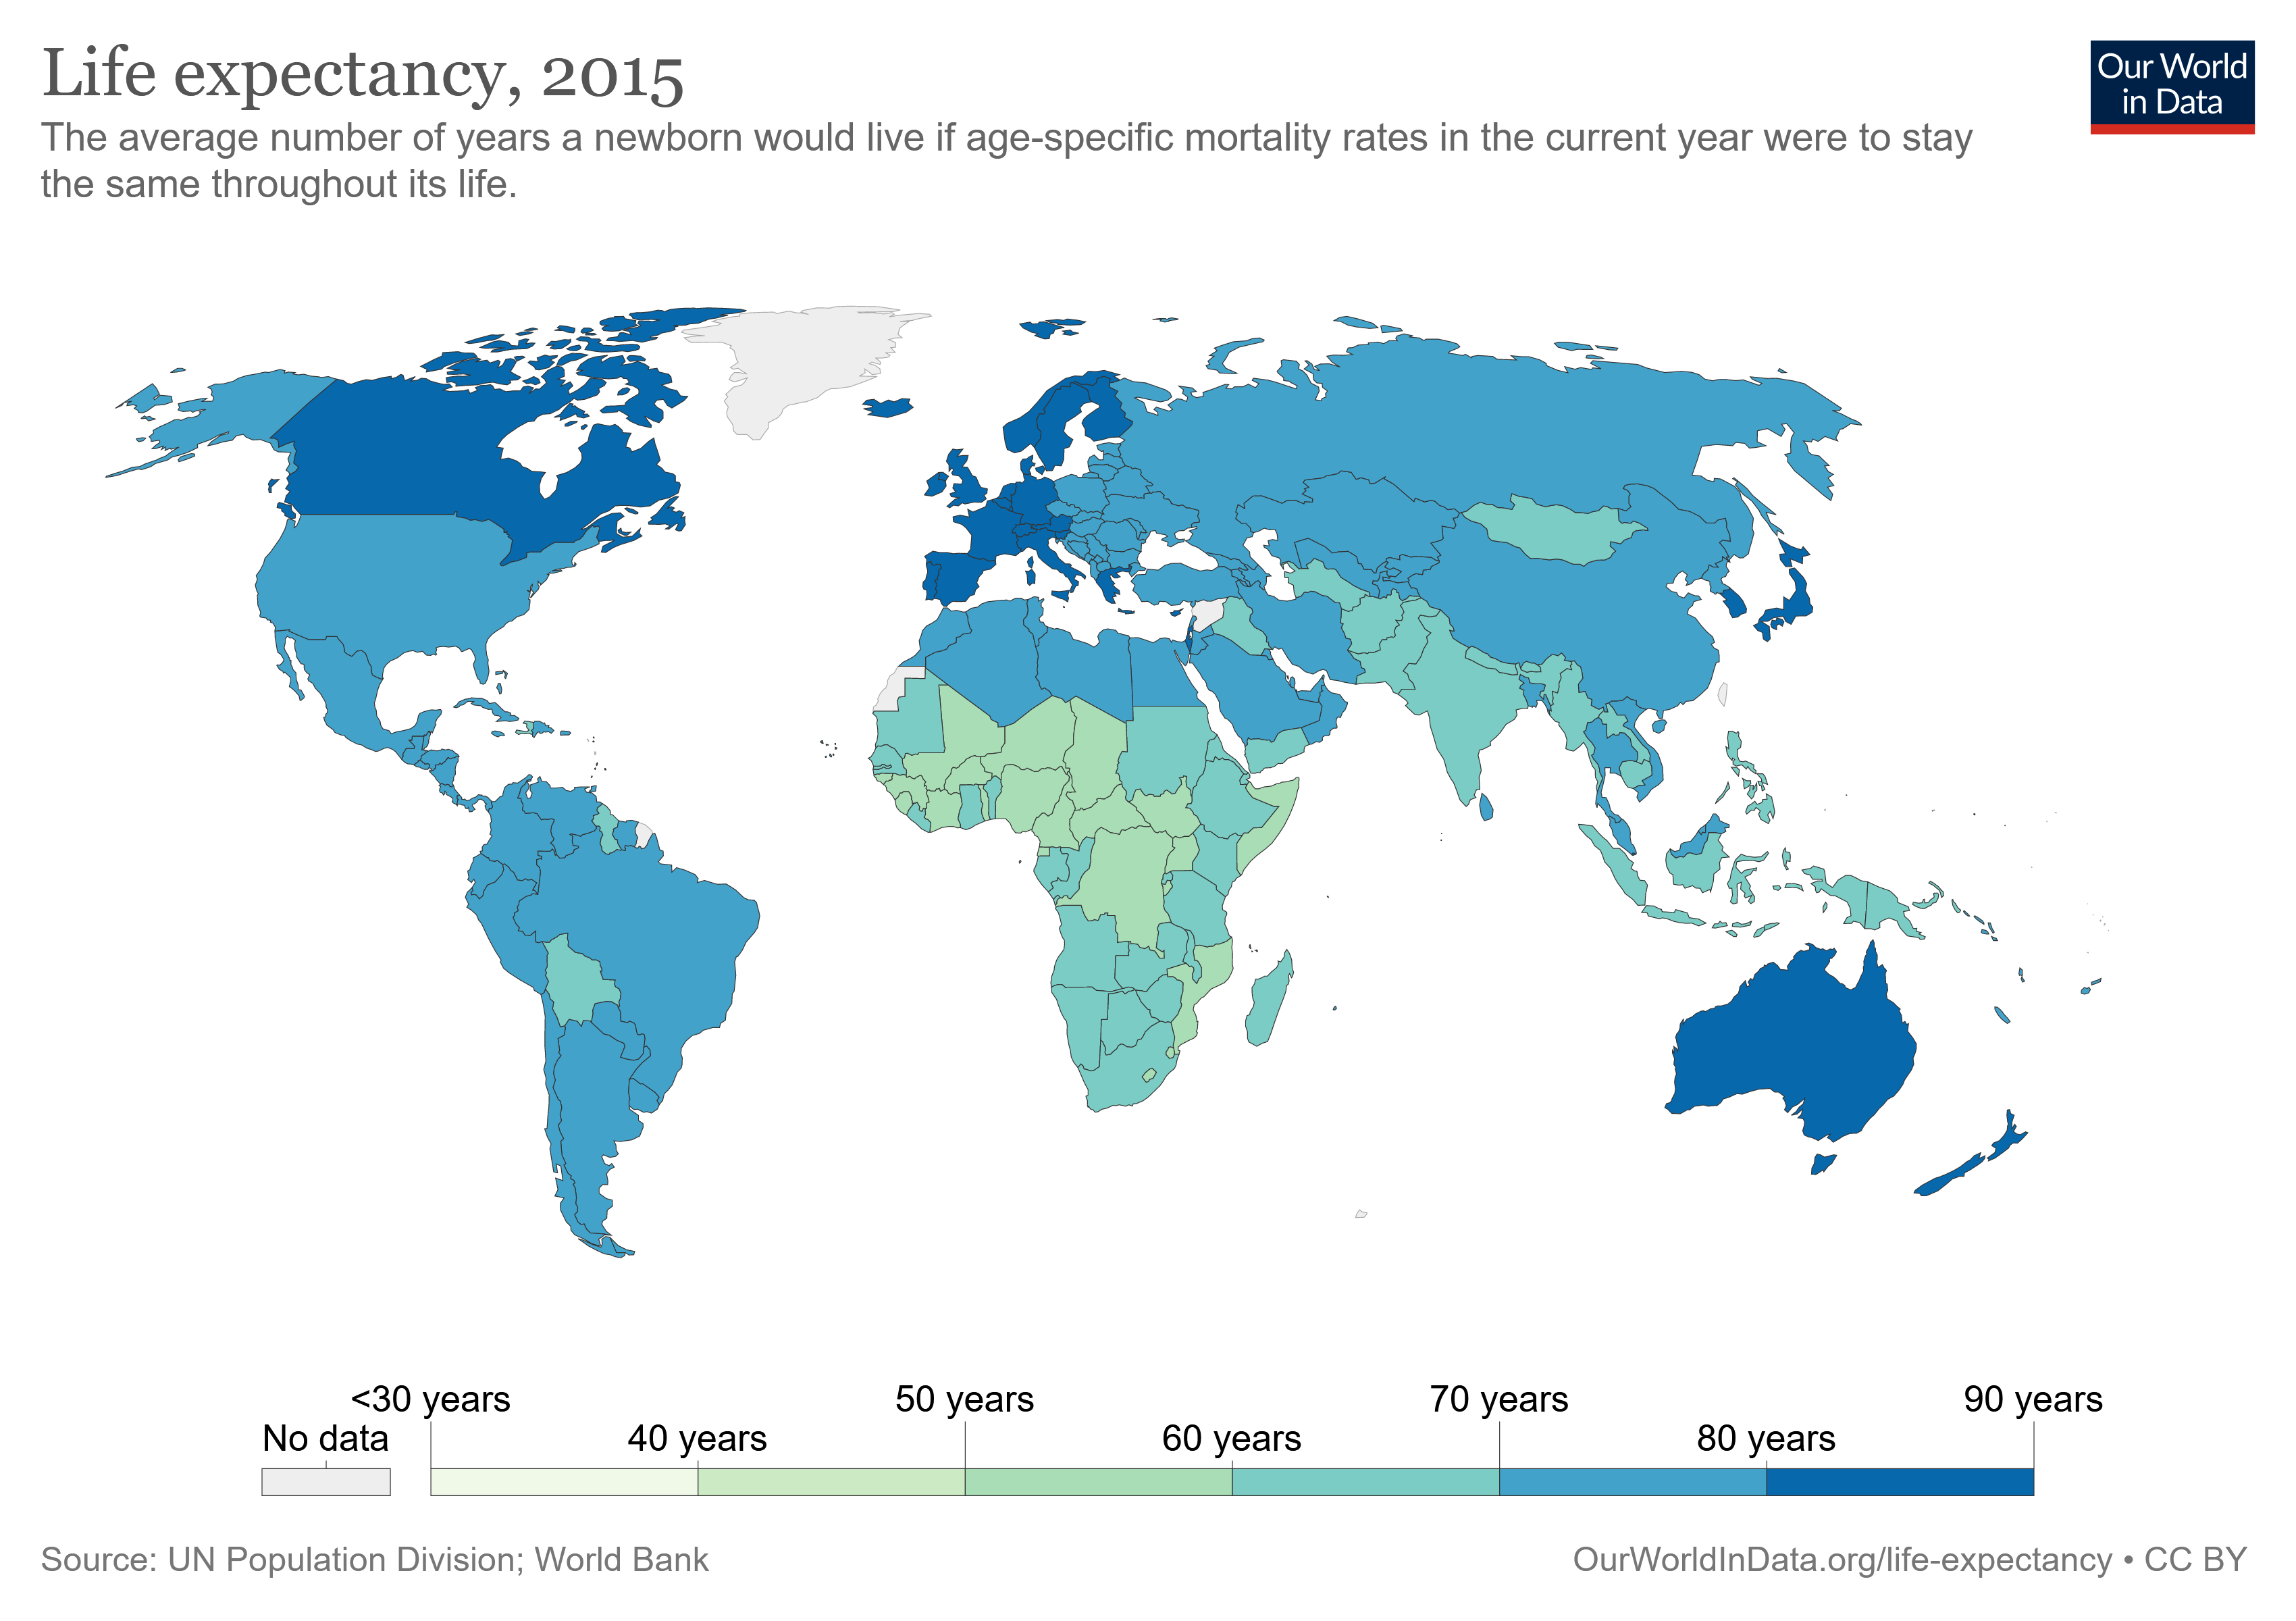
\includegraphics[height=3.2cm]{img/OWiD-life-expectancy.png}} \\
	\fbox{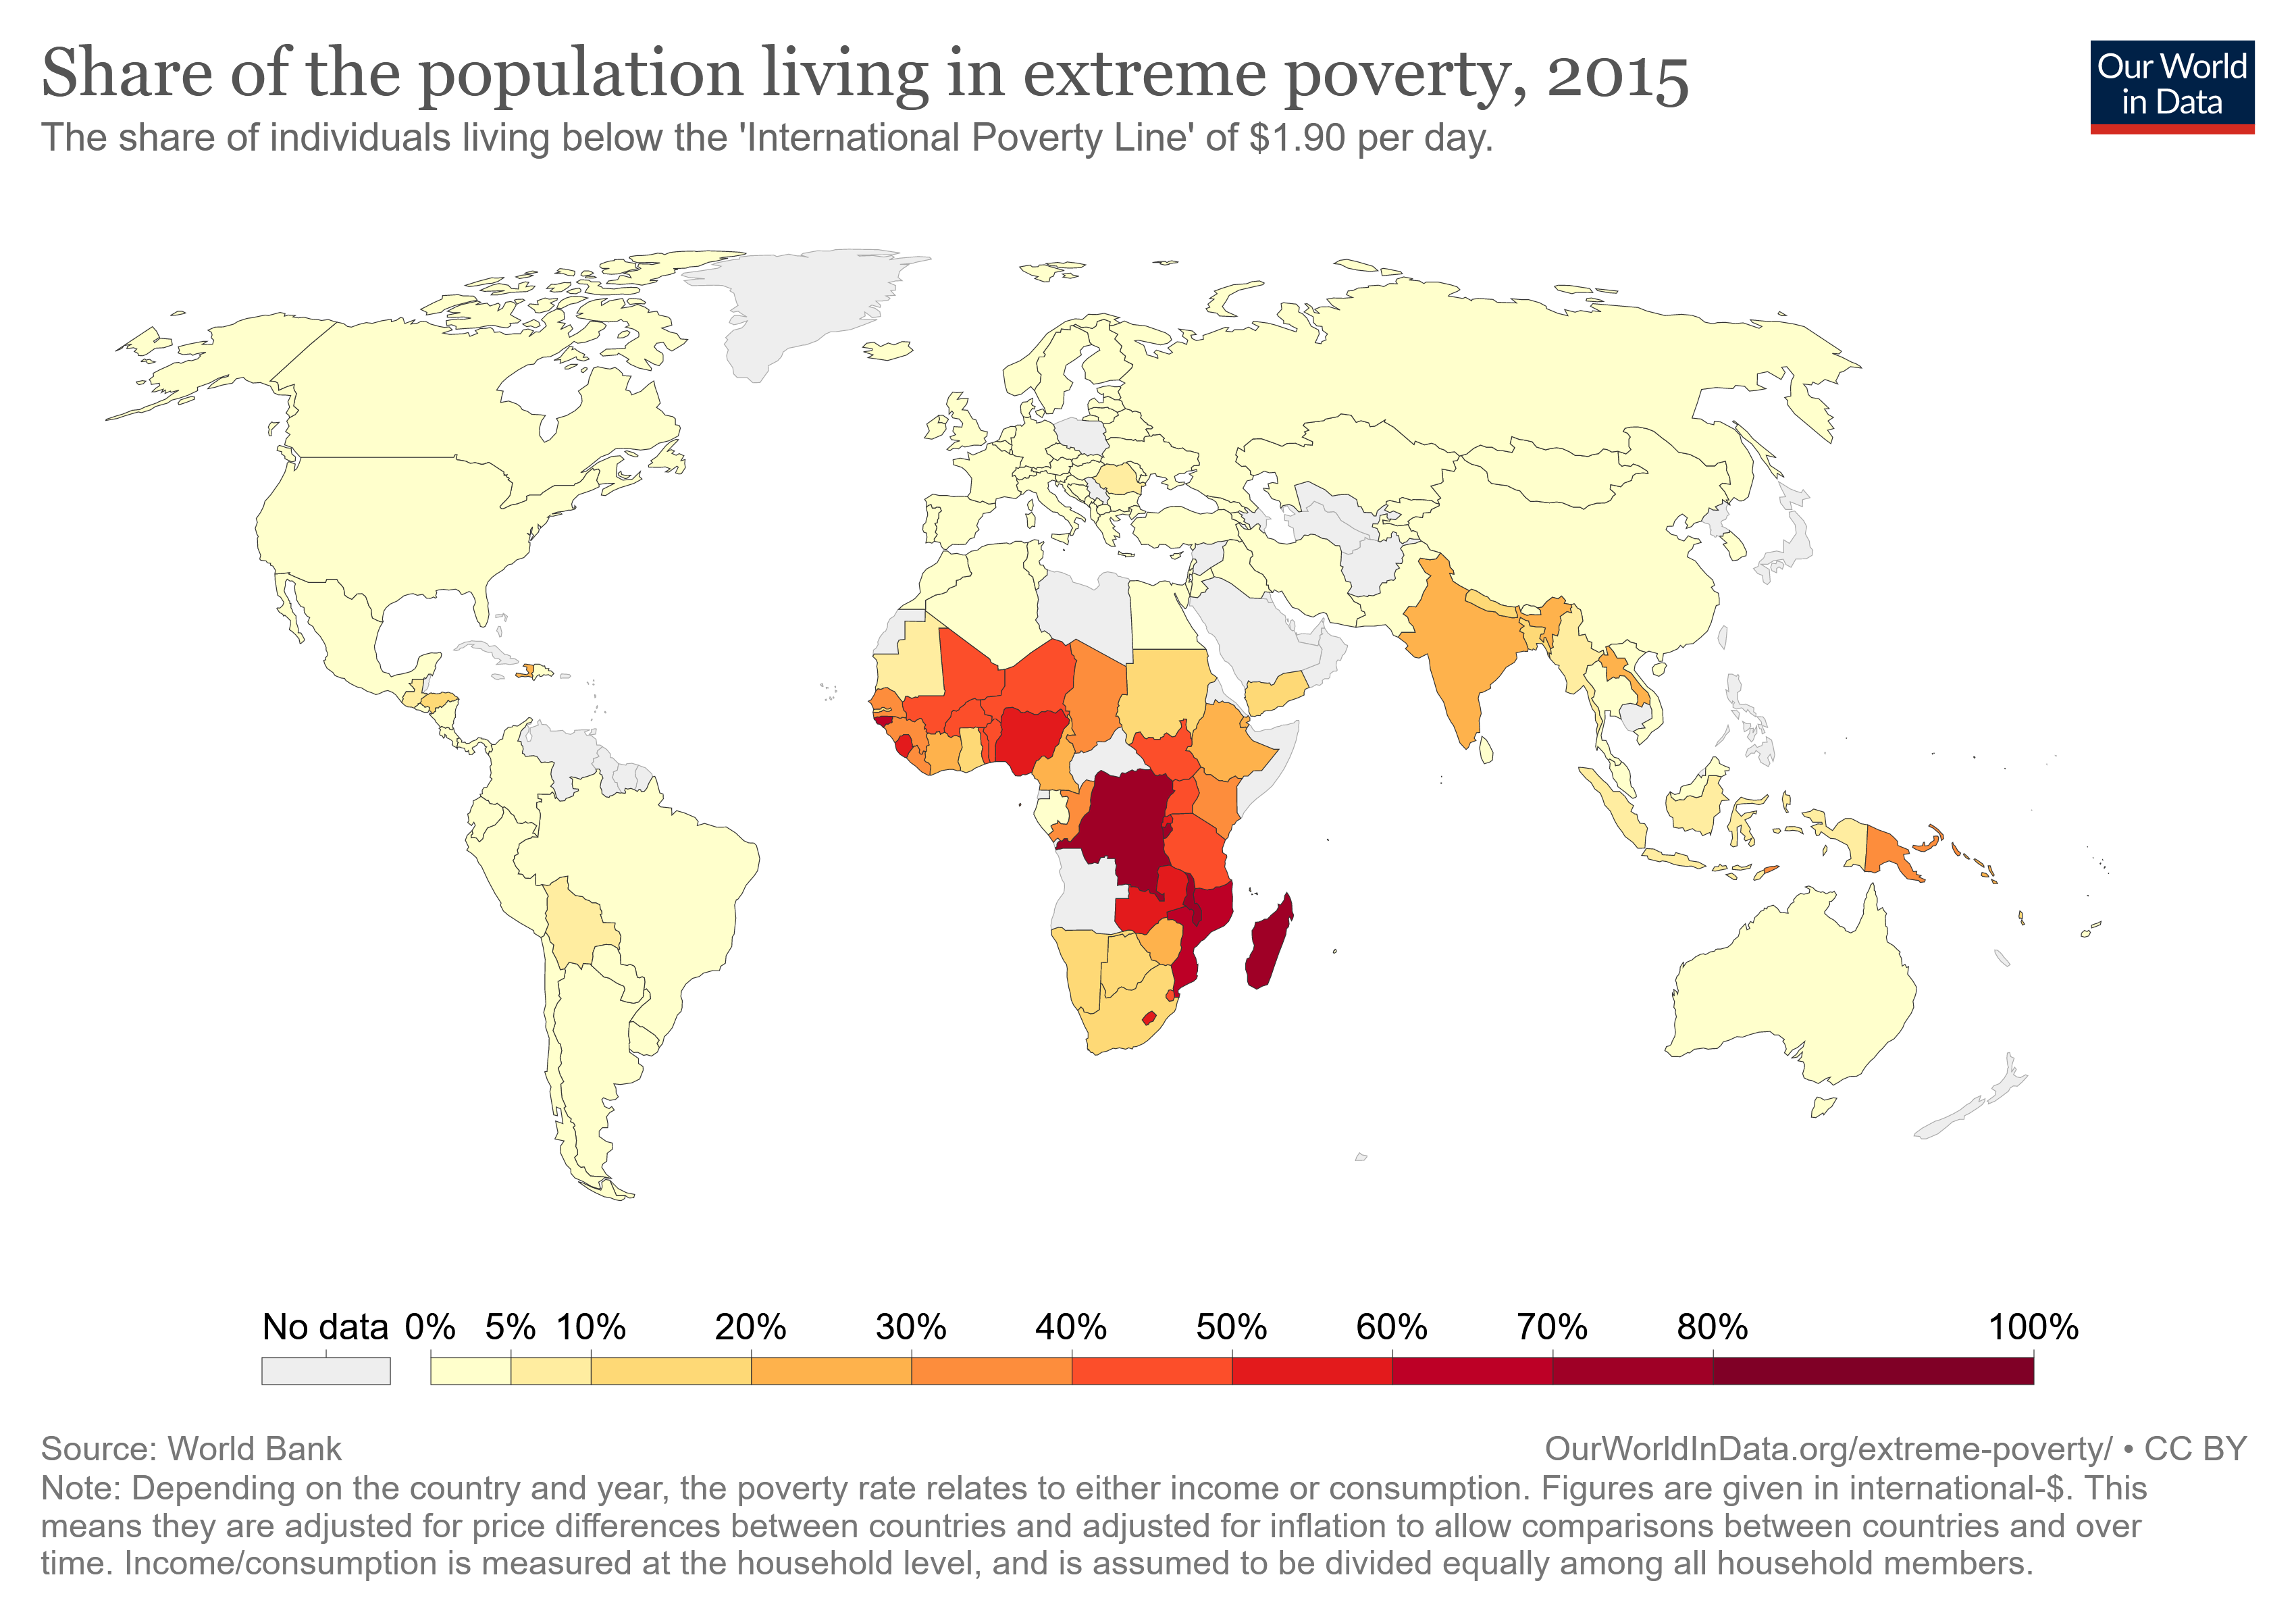
\includegraphics[height=3.2cm]{img/OWiD-extreme-poverty.png}} $\ \ $	\fbox{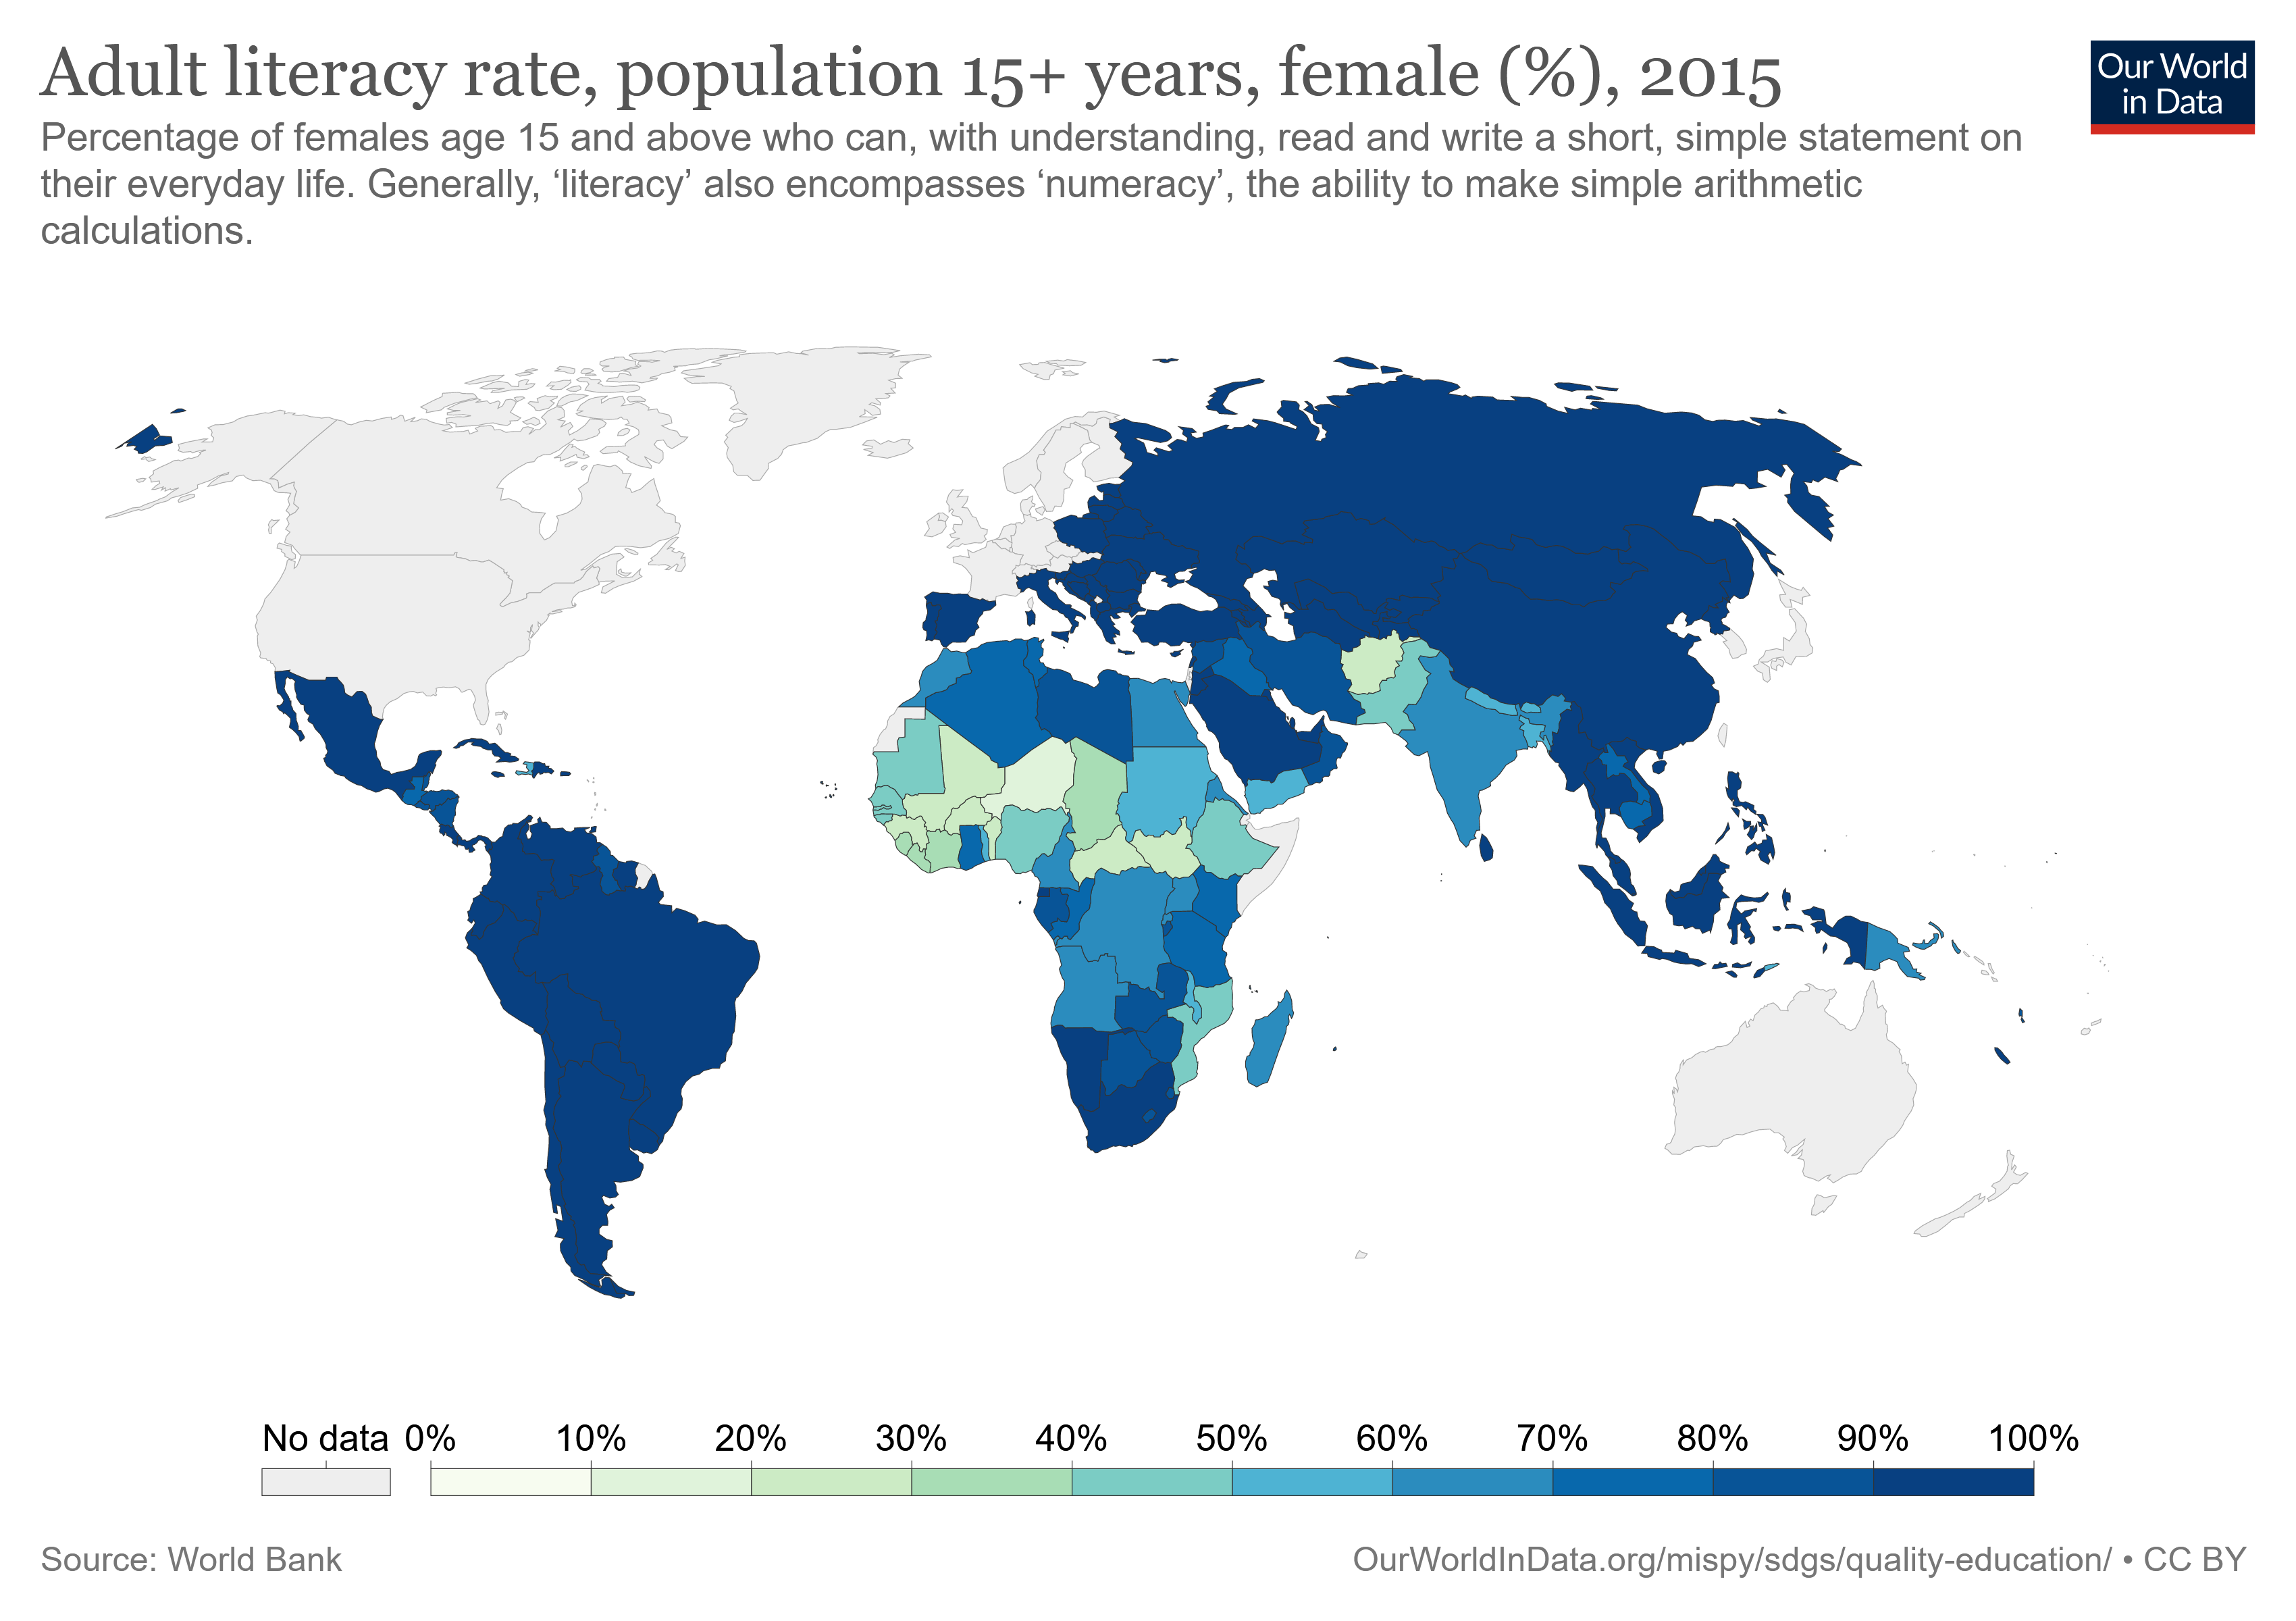
\includegraphics[height=3.2cm]{img/OWiD-literacy-female.png}} \\
	
	%	Between 1960 and 2015, developing countries received 4.15 trillion dollars in foreign aid 
\end{center}

\end{frame}



%%%%%%%%%%%%%%%%%%%%%%%%%%%%%%%%%%%%%%%%%%%%%%%%%%%%%%%%%%%%%%%%%%%%%

\begin{frame}{Did Aid Lead to Better Development Outcomes?}

\begin{center}
	\fbox{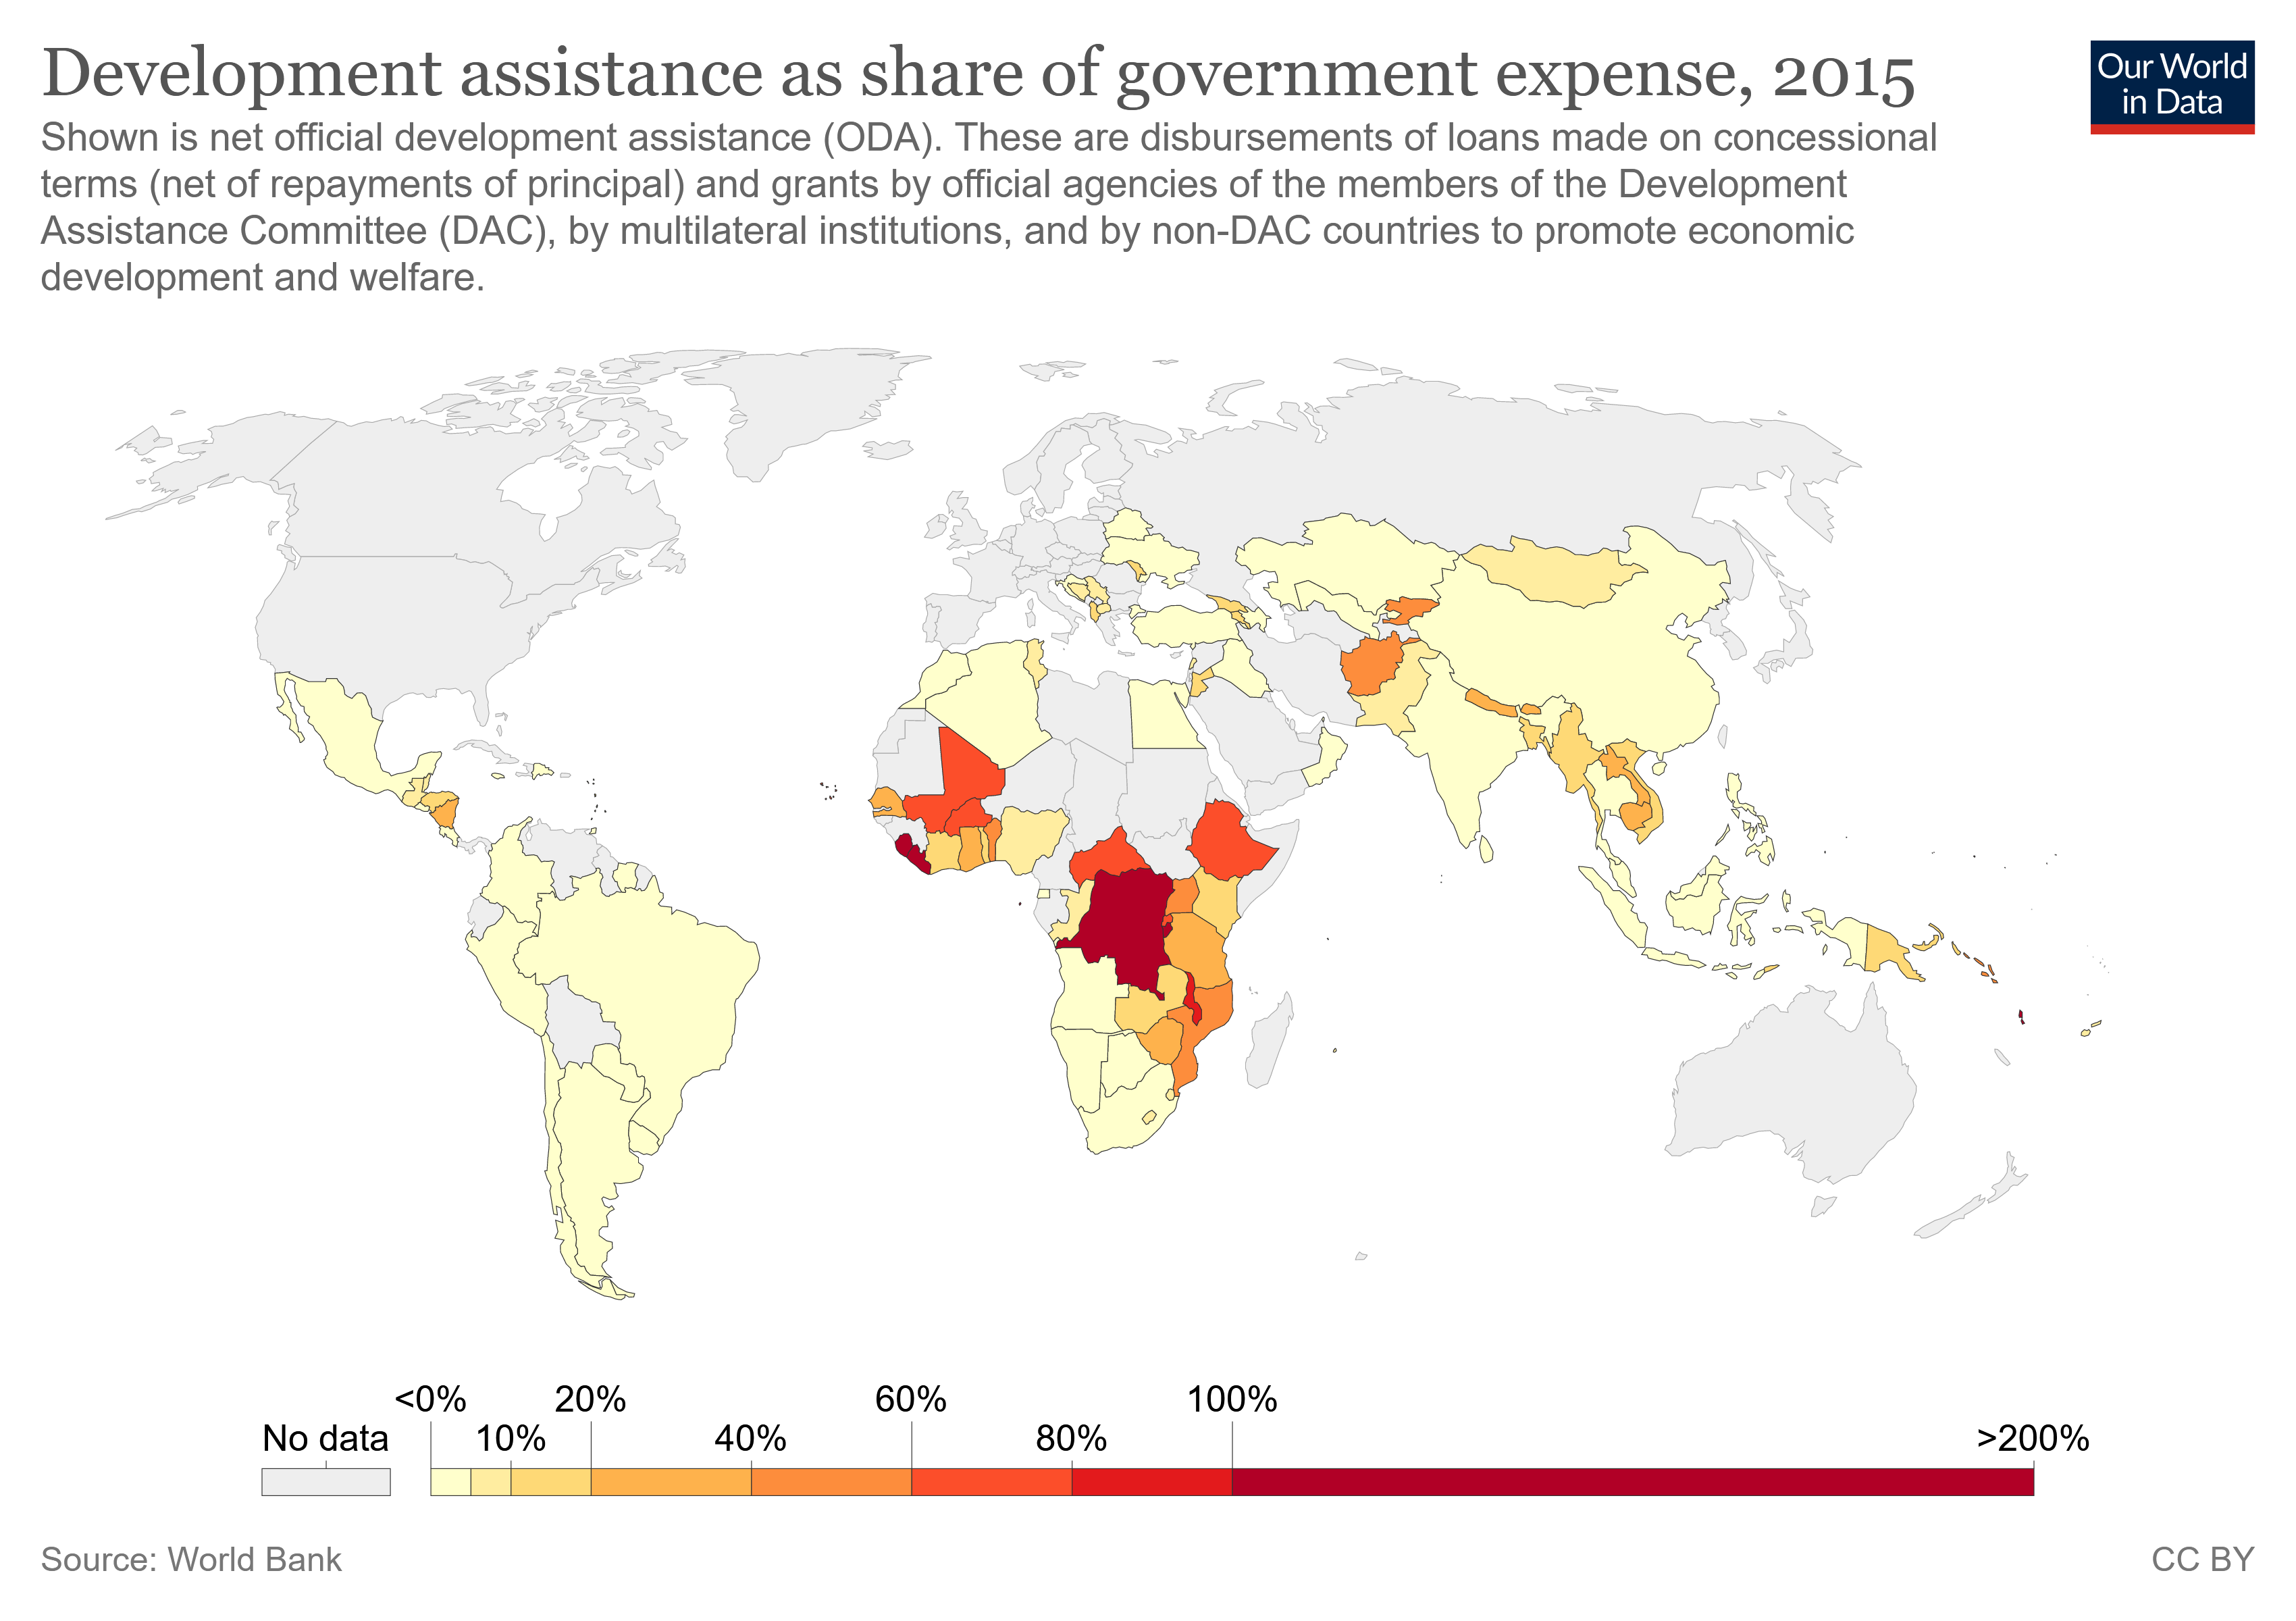
\includegraphics[height=4cm]{img/OWiD-aid-govt-expense-2015.png}} $\ \ $	\fbox{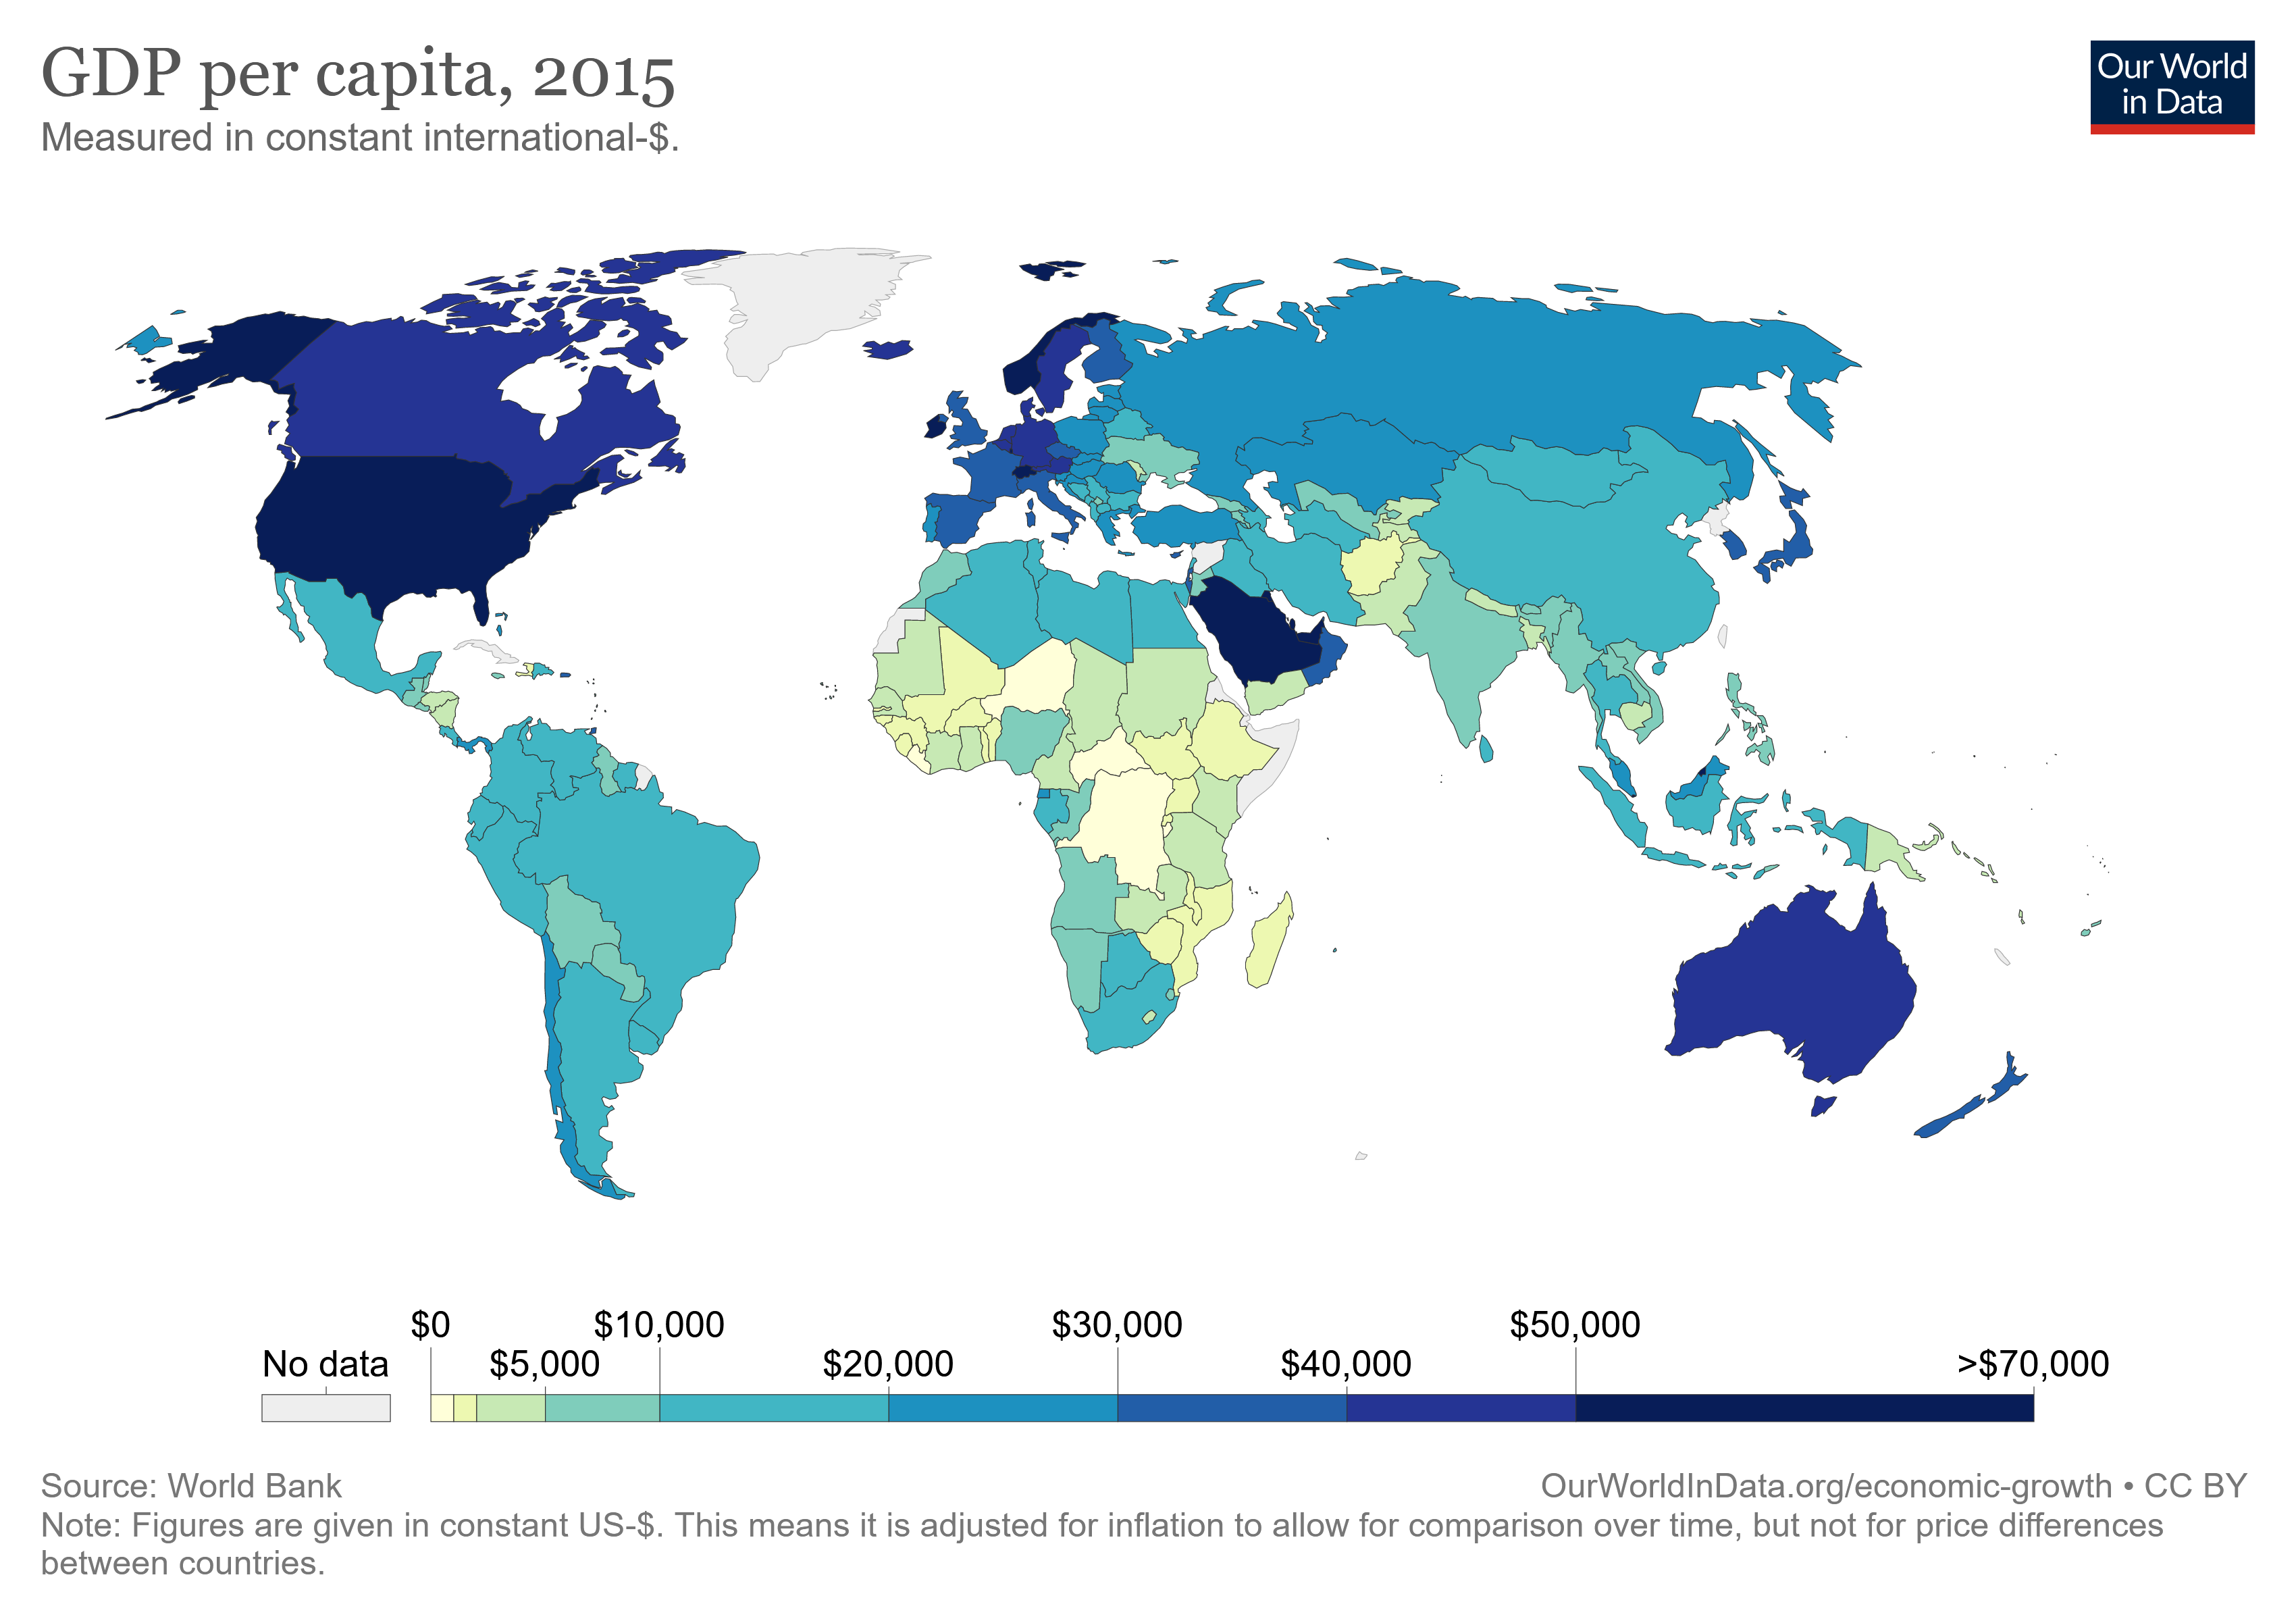
\includegraphics[height=4cm]{img/OWiD-gdp-per-capita.png}} \\
	
	\medskip
	\medskip
	
	Foreign aid pays for a large share of government expenditure in many of the poorest countries 
	
	\medskip
	\begin{itemize}
		
		\item In spite of billions of dollars in aid, many countries are not ``developed''
		
	\end{itemize}
\end{center}

\end{frame}


%%%%%%%%%%%%%%%%%%%%%%%%%%%%%%%%%%%%%%%%%%%%%%%%%%%%%%%%%%%%%%%%%%%%%

\begin{frame}{Did Aid Lead to Better Development Outcomes?}

\medskip
		Tanzania has received over 80 billion dollars in aid since 1960 (inflation adjust 2013 dollars)
	
\medskip
\begin{itemize}
		
		\item Some human development outcomes have improved since 1960:  life expectancy went up, both infant and maternal mortality declined, and educational attainment increased
		
\end{itemize}

\pause 
\medskip
\medskip
Would Tanzania have been better off without aid (or with less of it)?

\medskip
\begin{itemize}
	
	\item Argentina and Mongolia only received about 6.5 billion (2013) dollars in aid
	
	\medskip
	\begin{itemize}
		
		\item[$\Rightarrow$] Should we compare Tanzania to Argentina or Mongolia?
		
	\end{itemize}
	
\end{itemize}

\pause 
\medskip
\medskip
As Professor Duflo said:  we can't know what would have happened in Tanzania without aid


\end{frame}


%%%%%%%%%%%%%%%%%%%%%%%%%%%%%%%%%%%%%%%%%%%%%%%%%%%%%%%%%%%%%%%%%%%%%

\begin{frame}{What Can We Learn, and When Can We Learn It?}

\medskip
\textbf{An ``ideal'' experiment:} \\
Suppose Kenya, Tanzania, and Uganda all applied for a loan, but one got it (at random)

\medskip
\begin{itemize}
	
	\item No one is going to do this, and they (probably) shouldn't
	
	\item But such an experiment might help us learn about the impacts of aid on development
	
\end{itemize}

\pause
\medskip
\medskip
Some questions we might be able to answer:

\medskip
\begin{itemize}
	
	\item Do microfinance loan help women start small businesses and support their families?
	
	\item What were the impacts of school construction on education and adult wages?  
	
	\item Does subsidizing malaria treatment or bednets improve child health?  
	
\end{itemize}

\end{frame}




%%%%%%%%%%%%%%%%%%%%%%%%%%%%%%%%%%%%%%%%%%%%%%%%%%%%%%%%%%%%%%%%%%%%%%%%%%%

%\begin{frame}<handout:0>[bg,plain]
\begin{frame}[plain]

%\only<beamer>{\begin{adjustwidth}{0cm}{-4cm}}
	
	\begin{center}
		
		%\Large{\textcolor{white}{Budget Sets and Budget Lines}}
		\Large{\textcolor{williams}{The Other ``W'' Questions}}
		
	\end{center}
	
%	\only<beamer>{\end{adjustwidth}}
\end{frame}


%%%%%%%%%%%%%%%%%%%%%%%%%%%%%%%%%%%%%%%%%%%%%%%%%%%%%%%%%%%%%%%%%%%%%

\begin{frame}{Who?}

\medskip
Three types of individuals who often wish to initiate a program evaluation:

\medskip
\begin{itemize}
	
	\item Researchers, policymakers, donors
	
	\medskip
	\begin{itemize}
		
		\item Often asking different research questions
		
		\item All (policy-relevant) knowledge is (to some degee) context specific
		
	\end{itemize}
	
\end{itemize}

\medskip
\medskip
Who is interested in the results of a program evaluation?

\end{frame}


%%%%%%%%%%%%%%%%%%%%%%%%%%%%%%%%%%%%%%%%%%%%%%%%%%%%%%%%%%%%%%%%%%%%%

\begin{frame}{What?}

\medskip
Which programs \textbf{should} be evaluated?

\medskip
\begin{itemize}
	
	\item Is it replicable?
	
	\item Are there opportunity costs?
	
	\item Is it innovative or untested?  Do we care about the results?
	
\end{itemize}

\medskip
\medskip
When \textbf{shouldn't} a program be evaluated?  

\medskip
\begin{itemize}
	
	\item When are the opportunity costs low?
	
	\item When are the impacts of a program known?
	
	\item When is it unethical to have a comparison group?
	
\end{itemize}

\end{frame}


%%%%%%%%%%%%%%%%%%%%%%%%%%%%%%%%%%%%%%%%%%%%%%%%%%%%%%%%%%%%%%%%%%%%%

\begin{frame}{Where?}

\medskip
Program evaluation is a tool of both development and labor economics

\medskip
\begin{itemize}
	
	\item Randomized evaluations of social policy increasingly common in ``developed'' countries
	
	\item NGOs play an outsize role in service provision in LMICs
	
\end{itemize}

\pause
\medskip
\medskip
Certain countries may be over-represented (e.g.~Ghana, Kenya, Malawi)

\medskip
\begin{itemize}
	
	\item Where is data publicly available (cf.~Demographic and Health Surveys)?
	
	\item Other countries (e.g.~India, Indonesia) are large but \textbf{not} over-represented 
	
\end{itemize}

\pause
\medskip
\medskip
Where does aid go within countries?  Where do evaluations take place?

\medskip
\begin{itemize}
	
	\item Existing literature suggests aid ends up in wealthier places in poor countries
	
\end{itemize}

\end{frame}



%%%%%%%%%%%%%%%%%%%%%%%%%%%%%%%%%%%%%%%%%%%%%%%%%%%%%%%%%%%%%%%%%%%%%

\begin{frame}{When?}

\medskip
What are the differences between \textbf{retrospective} and \textbf{prospective} program evaluation?

\pause
\medskip
\begin{itemize}
	
	\item RCTs are not always prospective; quasi-experimental evaluations not always retrospective
	
	\medskip
	\begin{itemize}
		
		\item \textbf{Example:}  regression discontinuity design around eligibility cutoff
		
	\end{itemize}
	
\end{itemize}

\pause
\medskip
\medskip
What are (some of) the strengths of prospective evaluation?

\medskip
\begin{itemize}
	
	\item (I'm not going to tell you the answer, but Gertler et al.~have thoughts)
	
\end{itemize}

\pause
\medskip
\medskip
What are (some of) the (potential) weaknesses of prospective evaluation?

\pause
\medskip
\begin{itemize}
	
	\item External vs.~internal validity, (short) evaluation windows
	
\end{itemize}

\end{frame}






%%%%%%%%%%%%%%%%%%%%%%%%%%%%%%%%%%%%%%%%%%%%%%%%%%%%%%%%%%%%%%%%%%%%%%%%%%%

%\begin{frame}<handout:0>[bg,plain]
\begin{frame}[plain]

%\only<beamer>{\begin{adjustwidth}{0cm}{-4cm}}
	
	\begin{center}
		
		%\Large{\textcolor{white}{Budget Sets and Budget Lines}}
		\Large{\textcolor{williams}{How to Evaluate}}
		
	\end{center}
	
%	\only<beamer>{\end{adjustwidth}}
\end{frame}


%%%%%%%%%%%%%%%%%%%%%%%%%%%%%%%%%%%%%%%%%%%%%%%%%%%%%%%%%%%%%%%%%%%%%

\begin{frame}<handout:0>{How to Evaluate}

\medskip
\emph{This is what the whole rest of the class is about...}


\end{frame}




%%%%%%%%%%%%%%%%%%%%%%%%%%%%%%%%%%%%%%%%%%%%%%%%%%%%%%%%%%%%%%%%%%%%%

\begin{frame}{Three Questions}

\medskip
\begin{enumerate}
	
	\item What is the treatment?  What is $X$?
	
	\medskip
	\begin{itemize}
	
	\item Example:  \textbf{microfinance} (provision of small, uncollateralized loans to poor borrowers)
	
		\medskip
		\begin{itemize}
		
		\item Is the treatment a loan?  Or being offered a loan?  Or having an MFI in your neighborhood?
		
		\end{itemize}
	
	\item What is the \textbf{estimand}?  Difference treatments lead to different (expected) treatment effects
	
	\end{itemize}
	
	\pause
	\item What do we expect $X$ to impact?  What is $Y$?
	
	\medskip
	\begin{itemize}
	
	\item What are the outcomes, and how can/should we measure them?
	
	\item Example:  receiving a loan, having a microenterprise, HH income, empowerment, etc.
	
	\end{itemize}
	
	\pause
	\item How can we measure causal impacts of $X$?
	
	\medskip
	\begin{itemize}
		
		\item What is the \textbf{identification strategy}?  (some possible answers:  RCT, DD, IV, RD, ``HFB'')
		
	\end{itemize}
	
\end{enumerate}

\end{frame}


%%%%%%%%%%%%%%%%%%%%%%%%%%%%%%%%%%%%%%%%%%%%%%%%%%%%%%%%%%%%%%%%%%%%%%%

\begin{frame}<handout:0>{The Results Chain}

\begin{center}
	\begin{tikzpicture}
	
	% blank canvas
	\fill[fill=white,draw=white,ultra thin]
	(0,0) -- (14,0) -- (14,6) -- (0,6) -- cycle;
	%\draw[step=1.0,gray!20,thin] (0,0) grid (14,6);
	
	\node [anchor=north] (mike) at (7,5.8) {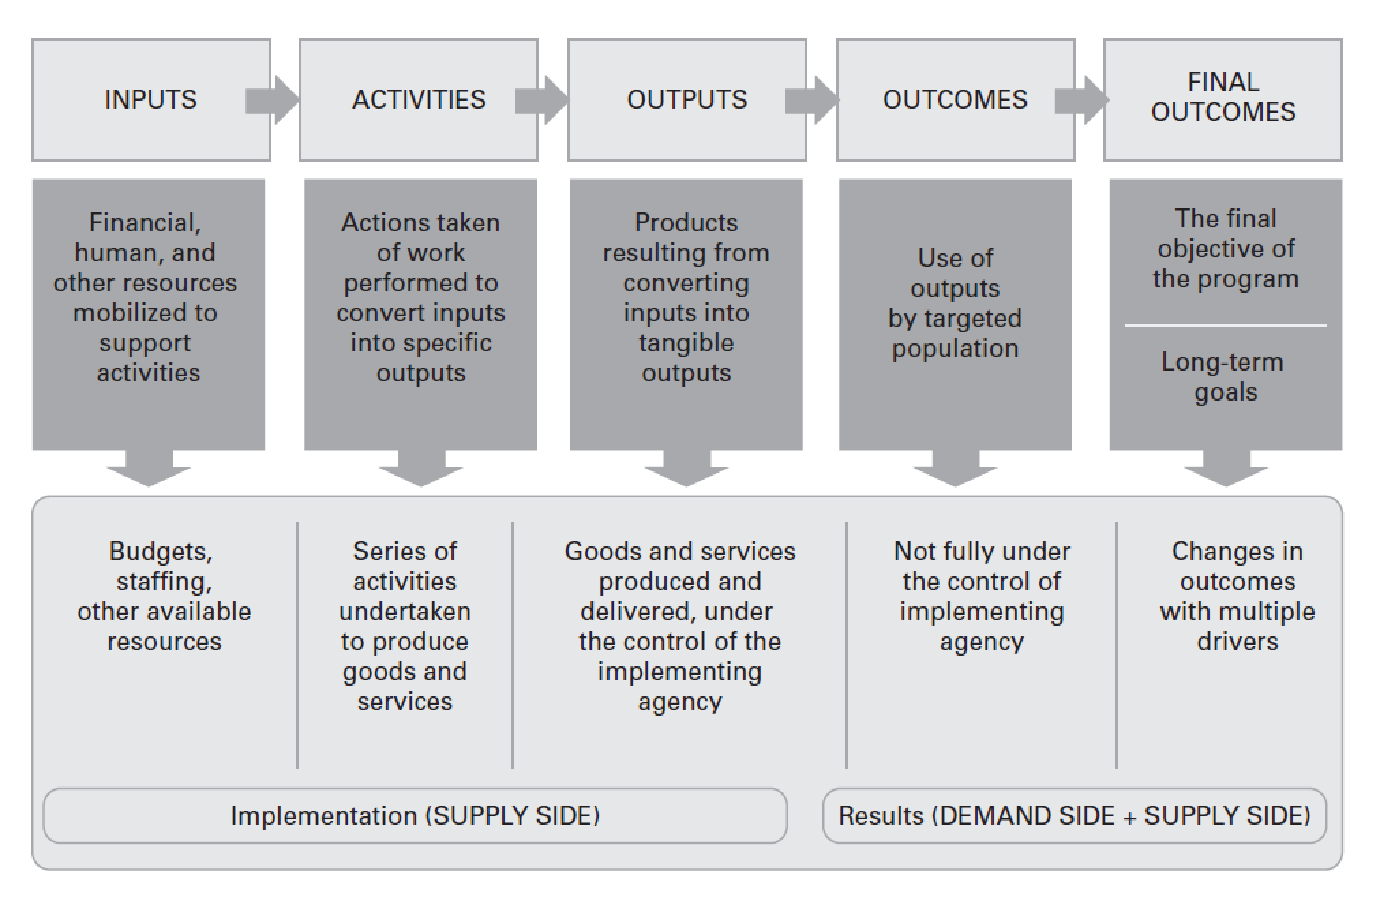
\includegraphics[height=5.6cm]{img/GertlerEtAl-results-chain}};

	
	\end{tikzpicture}
\end{center}
\end{frame}


%%%%%%%%%%%%%%%%%%%%%%%%%%%%%%%%%%%%%%%%%%%%%%%%%%%%%%%%%%%%%%%%%%%%%%%

\begin{frame}{The Results Chain}

\begin{center}
	\begin{tikzpicture}
	
	% blank canvas
	\fill[fill=white,draw=white,ultra thin]
	(0,0) -- (14,0) -- (14,6) -- (0,6) -- cycle;
	%\draw[step=1.0,gray!20,thin] (0,0) grid (14,6);
	
	\node [anchor=north] (mike) at (7,5.8) {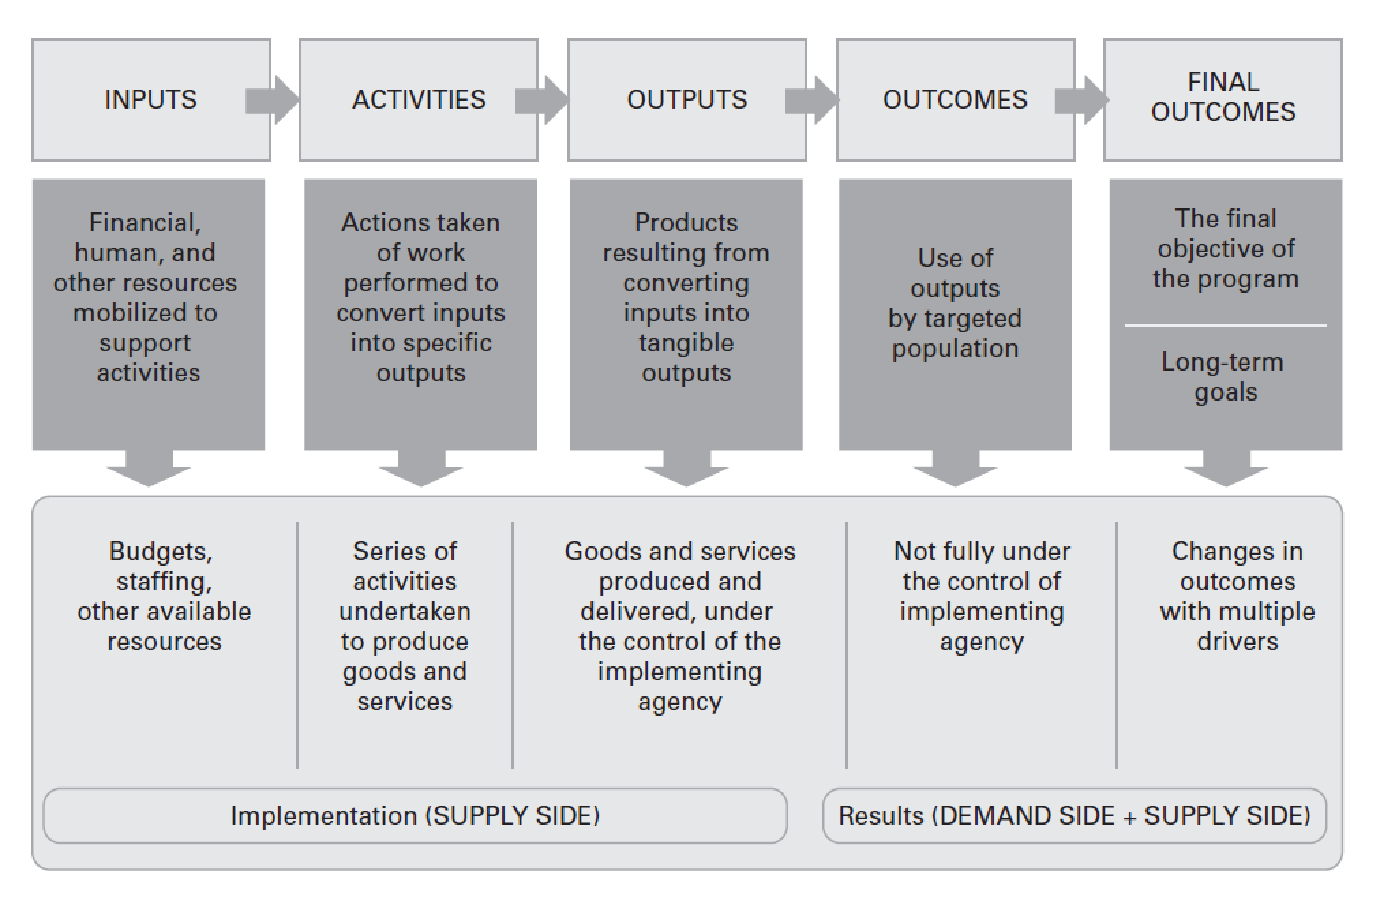
\includegraphics[height=5.6cm]{img/GertlerEtAl-results-chain}};
	
	\pgfmathsetmacro\mycolor{"oiblue"};
	\draw[\mycolor,thick] (0.1,0.1) -- (0.1,5.8) -- (7.75,5.8) -- (7.75,0.1) -- cycle;
	\node [\mycolor,anchor=east,font=\small] (text) at (2.875,5) {What is $X$?};
	
	\node [\mycolor,anchor=base east,font=\scriptsize] (text2) at ([yshift=-0.75cm]text.base east) {Research design?};
	\node [\mycolor,anchor=base east,font=\scriptsize] (text3) at ([yshift=-0.5cm]text2.base east) {Causal identification?};
	\node [\mycolor,anchor=base east,font=\scriptsize] (text4) at ([yshift=-0.5cm]text3.base east) {Estimand?};
	\node [\mycolor,anchor=base east,font=\scriptsize] (text5) at ([yshift=-0.5cm]text4.base east) {Implementation?};
	\node [\mycolor,anchor=base east,font=\scriptsize] (text6) at ([yshift=-0.5cm]text5.base east) {Compliance?};
	\node [\mycolor,anchor=base east,font=\scriptsize] (text7) at ([yshift=-0.5cm]text6.base east) {Contamination?};		
	
	\end{tikzpicture}
\end{center}
\end{frame}



%%%%%%%%%%%%%%%%%%%%%%%%%%%%%%%%%%%%%%%%%%%%%%%%%%%%%%%%%%%%%%%%%%%%%%%

\begin{frame}{The Results Chain}

\begin{center}
	\begin{tikzpicture}
	
	% blank canvas
	\fill[fill=white,draw=white,ultra thin]
	(0,0) -- (14,0) -- (14,6) -- (0,6) -- cycle;
	%\draw[step=1.0,gray!20,thin] (0,0) grid (14,6);
	
	\node [anchor=north] (mike) at (7,5.8) {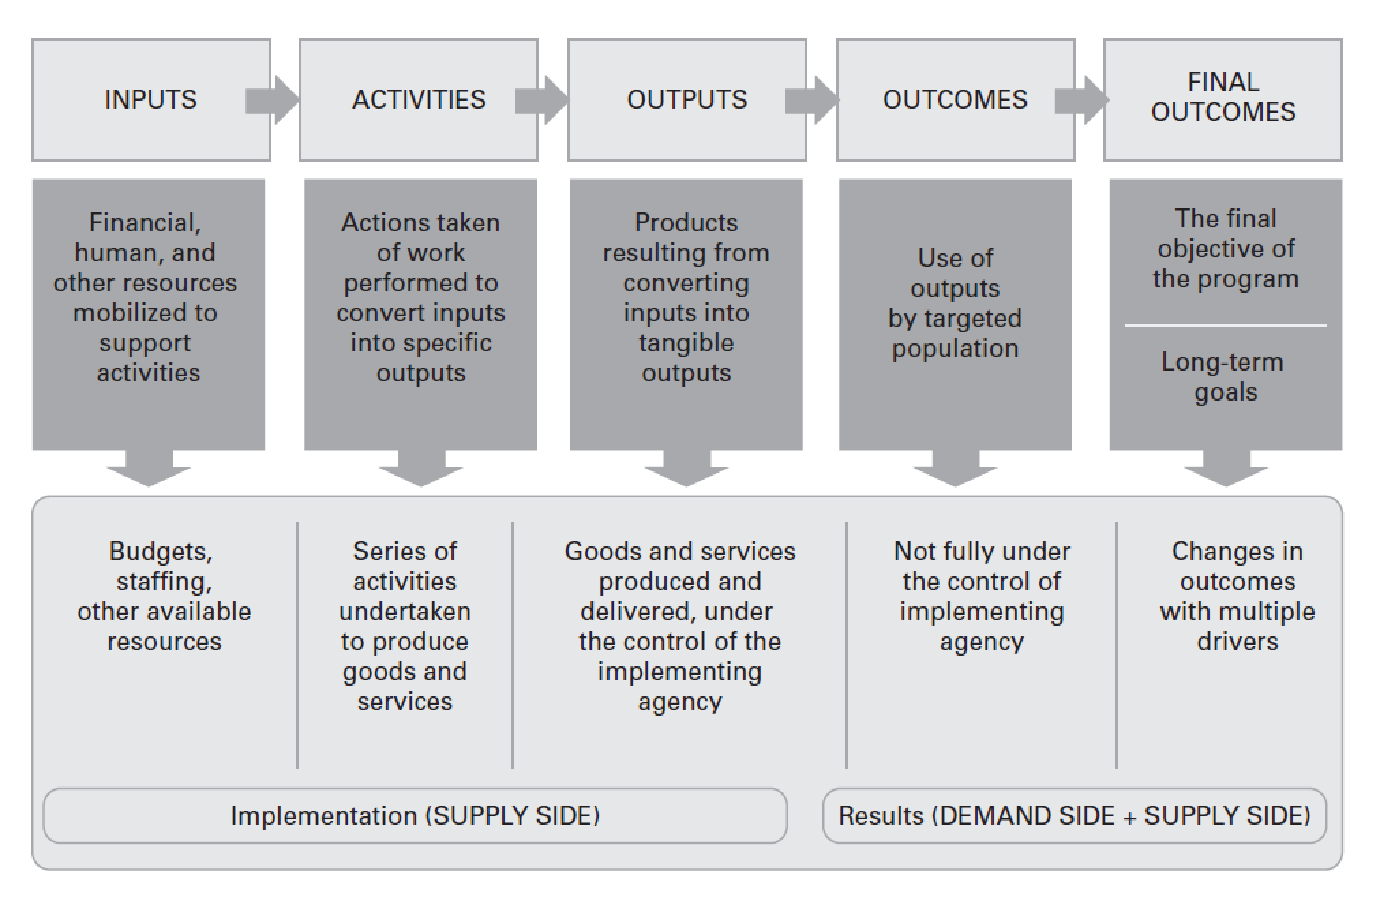
\includegraphics[height=5.6cm]{img/GertlerEtAl-results-chain.pdf}};
	
	\pgfmathsetmacro\mycolor{"gray!50"};
	\draw[\mycolor,thick] (0.1,0.1) -- (0.1,5.8) -- (7.75,5.8) -- (7.75,0.1) -- cycle;
	\node [\mycolor,anchor=east,font=\small] (text) at (2.875,5) {What is $X$?};
	
	\node [\mycolor,anchor=base east,font=\scriptsize] (text2) at ([yshift=-0.75cm]text.base east) {Research design?};
	\node [\mycolor,anchor=base east,font=\scriptsize] (text3) at ([yshift=-0.5cm]text2.base east) {Causal identification?};
	\node [\mycolor,anchor=base east,font=\scriptsize] (text4) at ([yshift=-0.5cm]text3.base east) {Estimand?};
	\node [\mycolor,anchor=base east,font=\scriptsize] (text5) at ([yshift=-0.5cm]text4.base east) {Implementation?};
	\node [\mycolor,anchor=base east,font=\scriptsize] (text6) at ([yshift=-0.5cm]text5.base east) {Compliance?};
	\node [\mycolor,anchor=base east,font=\scriptsize] (text7) at ([yshift=-0.5cm]text6.base east) {Contamination?};
	
	\pgfmathsetmacro\mycolor{"oiverm"};
	\draw[\mycolor,thick] (13.9,0.1) -- (13.9,5.8) -- (7.875,5.8) -- (7.875,0.1) -- cycle;
	\node [\mycolor,anchor=west,font=\small] (textB) at (11.125,5) {What is $Y$?};

	\node [\mycolor,anchor=base west,font=\scriptsize] (textB2) at ([yshift=-0.75cm]textB.base west) {Who is impacted?};	
	\node [\mycolor,anchor=base west,font=\scriptsize] (textB3) at ([yshift=-0.5cm]textB2.base west) {What outcomes?};	
	\node [\mycolor,anchor=base west,font=\scriptsize] (textB4) at ([yshift=-0.5cm]textB3.base west) {Timing of impacts?};	
	\node [\mycolor,anchor=base west,font=\scriptsize] (textB5) at ([yshift=-0.5cm]textB4.base west) {Measurement?};
	\node [\mycolor,anchor=base west,font=\scriptsize] (textB6) at ([yshift=-0.5cm]textB5.base west) {Effect size?};	
	\node [\mycolor,anchor=base west,font=\scriptsize] (textB7) at ([yshift=-0.5cm]textB6.base west) {Statistical power?};
	
	\end{tikzpicture}
\end{center}
\end{frame}




%%%%%%%%%%%%%%%%%%%%%%%%%%%%%%%%%%%%%%%%%%%%%%%%%%%%%%%%%%%%%%%%%%%%%

\begin{frame}{The Results Chain:  Examples}

\medskip
\textbf{Example 1:}  the World Bank funds the construction of new roads

\medskip
\medskip

\medskip
\textbf{Example 2:}  the Indonesian government builds thousands of new schools

\medskip
\medskip

\medskip
\textbf{Example 3:}  an NGO subsidizes effective treatment for malaria episodes


\end{frame}



%%%%%%%%%%%%%%%%%%%%%%%%%%%%%%%%%%%%%%%%%%%%%%%%%%%%%%%%%%%%%%%%%%%%%

\begin{frame}{Evaluating the Impacts of Subsidized Malaria Treatment}

\medskip
\begin{center}
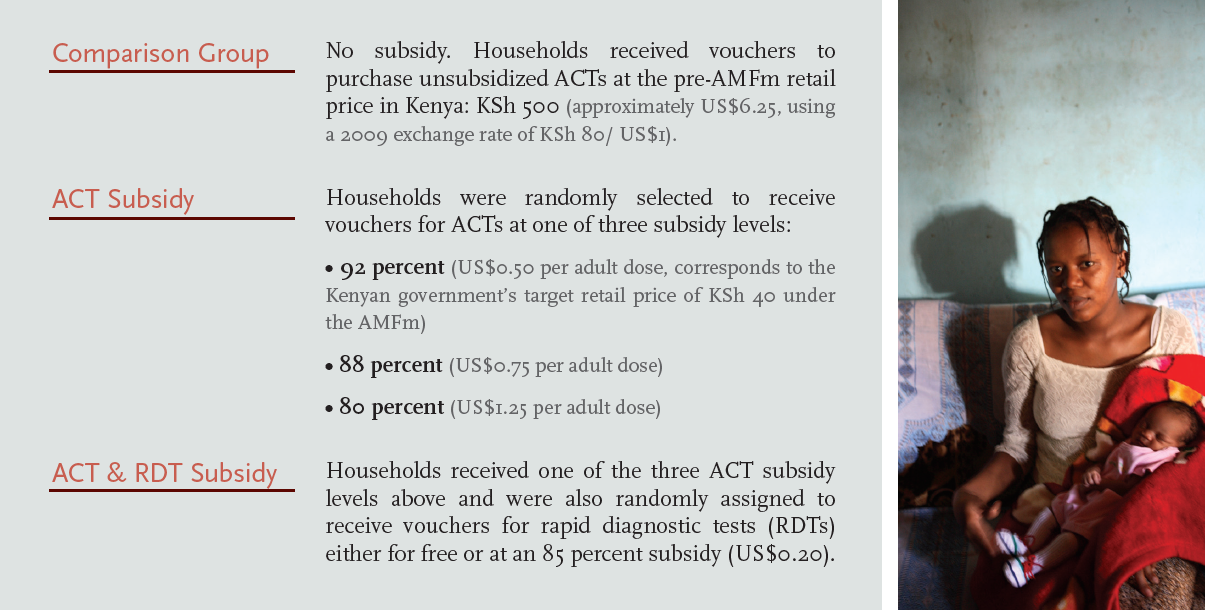
\includegraphics[height=5cm]{img/JPAL-ACT-desc.png}\\
\textcolor{gray}{\tiny{source:  J-PAL (photo:  Aude Guerrucci)}}
\end{center}

\end{frame}


%%%%%%%%%%%%%%%%%%%%%%%%%%%%%%%%%%%%%%%%%%%%%%%%%%%%%%%%%%%%%%%%%%%%%

\begin{frame}{Evaluating the Impacts of Subsidized Malaria Treatment}

\medskip
\begin{center}
	\fbox{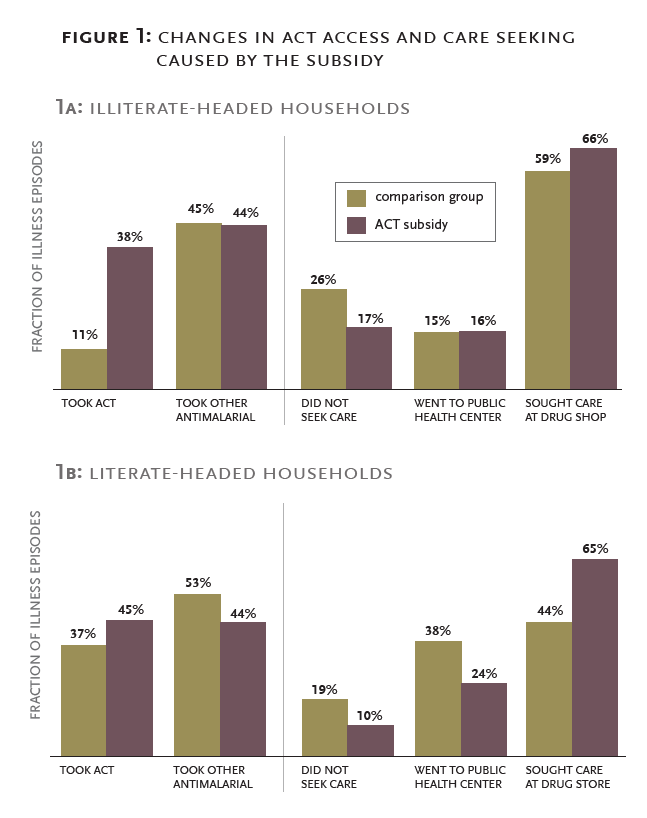
\includegraphics[height=5cm]{img/JPAL-ACT-Fig1.png}}\\
	\textcolor{gray}{\tiny{source:  J-PAL}}
\end{center}

\end{frame}


%%%%%%%%%%%%%%%%%%%%%%%%%%%%%%%%%%%%%%%%%%%%%%%%%%%%%%%%%%%%%%%%%%%%%

\begin{frame}{Evaluating the Impacts of Subsidized Malaria Treatment}

\medskip
\begin{center}
	\fbox{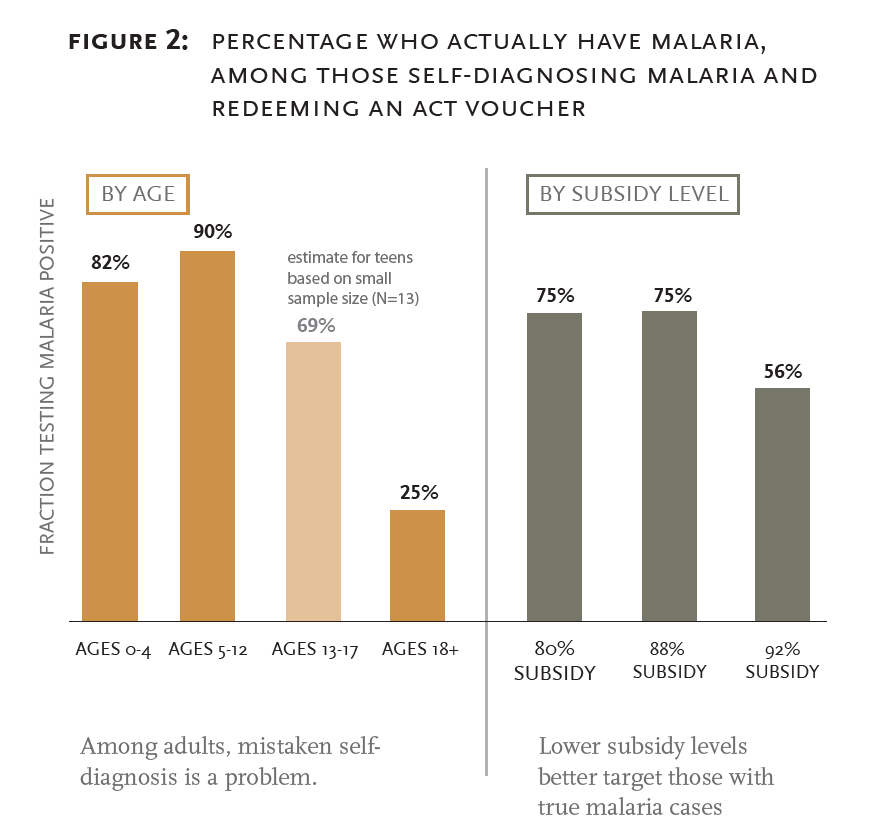
\includegraphics[height=5cm]{img/JPAL-ACT-Fig2.png}}\\
	\textcolor{gray}{\tiny{source:  J-PAL}}
\end{center}

\end{frame}


%%%%%%%%%%%%%%%%%%%%%%%%%%%%%%%%%%%%%%%%%%%%%%%%%%%%%%%%%%%%%%%%%%%%%

\begin{frame}{Evaluating the Impacts of Subsidized Malaria Treatment}

\medskip
\begin{center}
	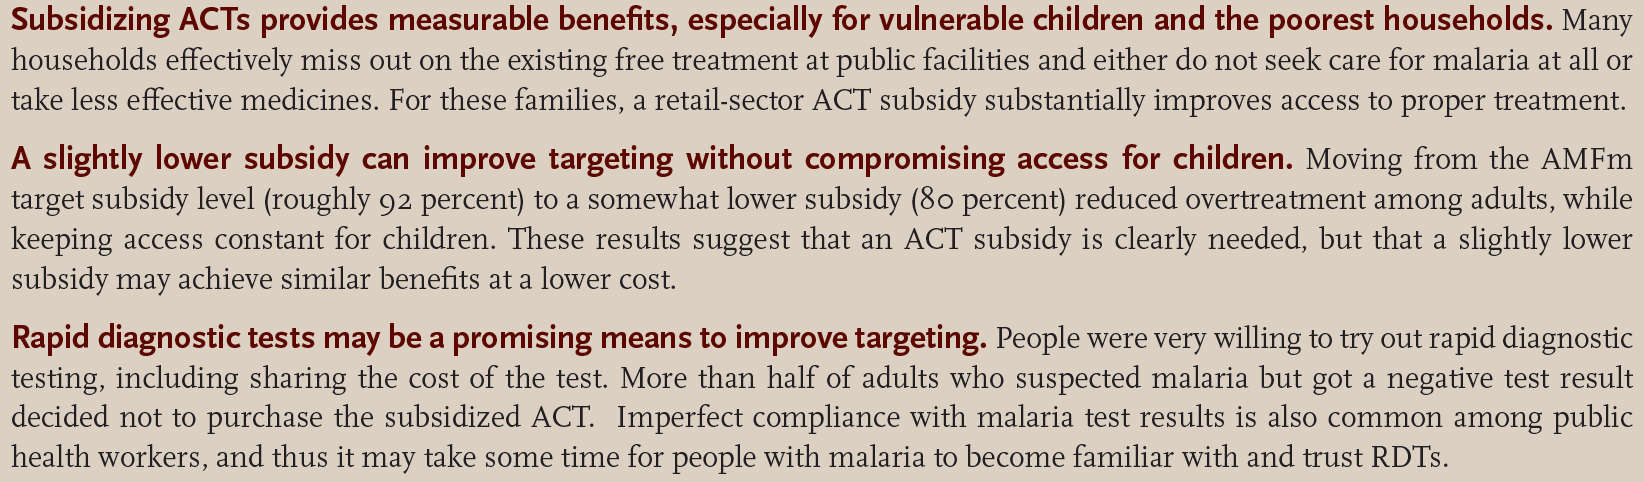
\includegraphics[width=12cm]{img/JPAL-ACT-conclusions.png}\\
	\textcolor{gray}{\tiny{source:  J-PAL}}
\end{center}

\end{frame}


\end{document}